\chapter{多元函数微分}
\label{chap:multivariate-differentiation}
\label{chap:multivariate-calculus}
\label{chap:multivariable-functions}

一元微分研究输入改变一点时输出改变多少：导数$f'(a)$是输出改变量与输入改变量之比的极限。许多量却同时依赖多个输入。平板上一点的温度由横、纵两个坐标决定，模型的损失由大量参数决定，流体的速度则在空间每一点给出一个向量。

以$f(x,y)=x^2+xy+y^2$为例，输入是平面上的点$(x,y)$，输出是一个实数。把$z=f(x,y)$看成地形的高度，把$(x,y)$看成地图上的位置。从一点出发，可以向东走、向北走、斜着走，也可以沿一条弯曲的路线靠近。本章要回答的问题是：能否用一个线性映射统一预测所有这些走法下的输出变化；这个预测在什么条件下成立；它的弯曲部分又怎样决定一点附近的形状，例如驻点是谷底、山顶还是鞍点。

第~\ref{chap:normed-inner-product-spaces}章已经建立了收敛、极限与连续性，证明了有限维空间中范数等价、完备，并定义了算子范数；伴随在第~\ref{chap:dual-spaces}章定义；第~\ref{chap:linear-representation}章给出了线性映射、多线性映射与对偶空间。这些是本章的语言。本章新增的问题是：能否把精确变化$f(\bm a+\bm h)-f(\bm a)$分成对$\bm h$线性的一阶部分和更小的余项。函数连续、有限变化有界，都不保证这样的分解存在。

各节按“对象—一阶—向量输出—高阶”的次序展开。第一节把多元函数看作位置上的标量场与向量场，回顾极限与连续性的要点。第二节从坐标方向的变化率出发，判断偏导数与方向导数何时组成全微分，再用内积把全微分表示为梯度，并用中值估计控制有限变化。

第三节把输出扩大为向量，用Jacobian矩阵记录微分，用链式法则组合复杂映射，并用导数的算子范数估计向量增量。第四节把微分再用于梯度，得到Hessian和多元Taylor公式，并据此判断驻点附近的形状；判断定性时要用到第~\ref{chap:eigen-spectral-decomposition}章的实对称谱分解。

本章只建立微分及其局部结论。以矩阵为自变量的微分在第~\ref{chap:matrix-differentiation}章，由方程隐式确定的函数在第~\ref{chap:implicit-inverse-functions}章；导数怎样控制误差放大、一阶预测在有限步长下还差多少，集中在第~\ref{chap:differential-perturbation-analysis}章。本章还沿用第~\ref{chap:linear-operations}章的向量、矩阵与行列式，以及一元微分的结论，可参考\BookChapterRef{chap:univariate-differentiation}{卷一“一元函数的微分”章}。偏导数与局部线性近似的直观介绍可参考\scite{math-openstax-calculus3}，严格的多元微分论证可参考\scite{math-lebl2026analysis2}。

\par\Needspace{14\baselineskip}

\label{sec:analysis-multivariable-differentiation}
\label{sec:multivariable-differentiation}

\section{多元函数与场}
\label{sec:multivariable-functions-and-fields}

微分和积分都要先说清研究的是什么函数。本部分最常见的情形是：空间中每个位置都带着一个可以测量的量。平板上每一点有温度，河水中每一点有流速，金属块中每一点有密度。这样的量随位置变化，输入是位置的坐标，输出是该位置上读出的量。

第~\ref{sec:multivariable-joint-limit-section}节已经从极限的角度定义了多元标量函数与向量值映射。本节换一个角度，把它们看作空间位置上的属性：先按输出是一个数还是一个向量，区分标量场与向量场；再说明本部分的定义域、输出空间以及极限与连续性怎样理解。这些约定确定了后面各章微分与累计的对象。

\subsection{标量场}
\label{sec:multivariable-scalar-fields}

温度计放在平板的不同位置，读数不同；把每个位置与它的读数配对，就得到一个函数。密度、压强、电势也都在每个位置给出一个实数。这类函数在每个位置只给出大小，不带方向。
\begin{definition}[标量场]
\label{def:multivariable-scalar-field}
设$\Omega\subseteq\mathbb R^d$。映射$f:\Omega\to\mathbb R$称为$\Omega$上的\term{标量场}（scalar field）；它把每个位置$\bm x\in\Omega$映为一个实数$f(\bm x)$。
\end{definition}
作为映射，标量场就是定义~\ref{def:multivariable-scalar-function}中的多元标量函数。“场”这个名称只强调输入是空间位置、输出是该位置的属性。后面称它为多元函数还是标量场，取决于讨论的是一般的输入输出关系，还是位置上的物理量，数学内容相同。

以$f(x,y)=x^2+y^2$为例，它在每个位置给出到原点距离的平方。它有两种画法。第一种画法把函数值当作高度，得到三维空间中的曲面$z=x^2+y^2$，形状像一只碗。第二种画法留在输入平面里，画出等值曲线$\{(x,y):x^2+y^2=c\}$。

对这个函数，$c>0$时等值曲线是半径为$\sqrt c$的圆，$c=0$时只剩原点，$c<0$时是空集。取$c=1,2,3,4$，半径依次为$1,\sqrt2\approx1.41,\sqrt3\approx1.73,2$，相邻两圈的间距越来越小。函数值每增加$1$所需走的距离越来越短，说明离原点越远，场值沿径向增长得越快。

这一观察还只是定性的。度量“沿某方向增长多快”需要导数：第~\ref{sec:multivariable-gradient-inner-product}节把它写成梯度，并说明梯度与等值曲线正交。

\subsection{向量场}
\label{sec:multivariable-vector-fields}

河水在每一点有流速，物体在重力场或电场中的每一点受力。这些量既有大小又有方向，并且与位置同处一个空间：流速可以画成从该点出发的箭头。
\begin{definition}[向量场]
\label{def:multivariable-vector-field}
设$\Omega\subseteq\mathbb R^d$。映射$\bm F:\Omega\to\mathbb R^d$称为$\Omega$上的\term{向量场}（vector field）。按本书约定，$\bm F(\bm x)$写成$d\times1$列矩阵$(F_1(\bm x),\ldots,F_d(\bm x))^\top$，每个分量$F_i:\Omega\to\mathbb R$都是标量场。
\end{definition}
向量场的输入是位置，输出是放在该位置的一个向量。例如$\bm F(x,y)=(x,y)^\top$的箭头从原点向外，离原点越远越长；$\bm F(x,y)=(-y,x)^\top$的箭头与以原点为圆心的圆相切，按逆时针方向。第~\ref{chap:path-integrals}章用这两个场比较沿路径做的功。

向量场是向量值函数的特例。一般向量值函数$F:\Omega\subseteq\mathbb R^d\to\mathbb R^m$的输出维数$m$可以与输入维数不同：参数曲线把一个参数映为空间中的点，神经网络的一层把输入向量映为另一维数的向量。向量场要求$m=d$，输出向量才能画成输入空间中的箭头，也才能与路径的切向量或曲面的法向量作内积。

输出还可以是矩阵。若每个位置给出一个$p\times q$矩阵，例如介质中每一点的应力矩阵，就得到矩阵值的场；它的每个元素仍是标量场。第~\ref{chap:matrix-differentiation}章研究的则是另一种情形：输入本身是矩阵，例如$\bm X\mapsto\bm X^{-1}$。判断一个映射属于哪一类时，要分别核对输入空间和输出空间，不能只看表达式里是否出现矩阵。

\subsection{多元函数的极限与连续}
\label{sec:multivariable-field-limits-continuity}

标量场和向量场的极限与连续性已在第~\ref{chap:normed-inner-product-spaces}章建立，这里只回顾后面要用的结论，不重复证明。

极限用输入、输出空间的范数定义（定义~\ref{def:multivariable-limit}）。$\lim_{\bm x\to\bm a}F(\bm x)=\bm L$的意思是：只要输入进入以$\bm a$为心的某个去心小球，输出与$\bm L$的距离就小于给定误差，不论输入沿什么路线进入。连续性（定义~\ref{def:multivariable-scalar-continuity}）要求这个极限等于$F(\bm a)$。

对有限维的向量输出，这些判断可以逐分量进行：向量场或矩阵值的场在一点有极限或连续，当且仅当每个输出分量如此（定理~\ref{thm:multivariable-coordinatewise-convergence}）。逐分量分解的是输出。输入的多个坐标不能这样拆开，因为输入可以同时改变全部坐标、沿弯曲的路线趋近。

因此，沿路径检验只能用来否定极限。沿两条路径得到不同的极限值，联合极限就不存在：示例~\ref{ex:multivariable-path-limits}中的$xy/(x^2+y^2)$沿$x$轴趋于$0$，沿$y=x$趋于$1/2$。反过来，只检查若干条路径不能证明极限存在：示例~\ref{ex:multivariable-parabola-path-limit}中的$x^2y/(x^4+y^2)$沿每条直线都趋于$0$，沿抛物线$y=x^2$却恒为$1/2$。要证明极限存在，需要一个只依赖输入到基点距离的统一误差估计。

这个区别在微分中还会出现。方向导数是沿固定直线取的极限，全微分则要求误差对全部趋近方式统一受控；第~\ref{sec:multivariable-total-differentiation}节的反例与上面的抛物线例子结构相同。

最后约定定义域。讨论微分时，基点取在开集内部，从基点出发向任何方向走足够小的一步都不离开定义域；讨论积分时，累计范围通常是有界闭区域，这时只要求被积函数在区域上连续或满足相应的可积条件。

\section{多元标量函数的一阶微分}
\label{sec:multivariable-scalar-first-order}

上一节回顾的极限与连续只问函数值是否趋近，本节开始度量函数值变化的快慢。最直接的办法是沿一条直线把多元函数变成一元函数，再求一元导数，这样得到偏导数和方向导数。

偏导数和方向导数只描述固定直线上的变化。接下来要判断，这些方向信息何时组成一个对全部小扰动都有效的线性近似，即全微分。全微分是作用于输入扰动的线性泛函；借助对偶空间与内积，它可以由输入空间中的一个向量表示，这个向量就是梯度。最后沿线段使用一元中值定理，把梯度的大小转化为有限变化的界。

本节研究实值函数$f:U\subseteq\mathbb R^d\to\mathbb R$，并要求$U$为开集。开集中每一点都有一个含于$U$的小球，从基点出发向任何方向走足够小的一步仍在定义域内，双侧差商因而都有意义。

\subsection{偏导数与方向导数}

固定除$x_j$以外的全部坐标，$f$就变成只依赖$x_j$的一元函数，它的导数就是偏导数。
\begin{definition}[偏导数]
\label{def:multivariable-partial-derivative}
设$\bm a\in U$，令$\bm e_j$是第$j$个坐标为$1$、其余为$0$的向量。若双侧极限
\[
 \partial_jf(\bm a)=\frac{\partial f}{\partial x_j}(\bm a)
 =\lim_{t\to0}\frac{f(\bm a+t\bm e_j)-f(\bm a)}t
\]
存在且有限，就称它为$f$在$\bm a$处关于$x_j$的\term{偏导数}（partial derivative）。
\end{definition}
偏导数是只改变第$j$个坐标、其余坐标固定时的变化率。符号$\partial$提醒我们，这里求的是一个坐标切片的导数。
对二元函数，$\partial_xf(a,b)$是用竖直平面$y=b$截曲面所得曲线在$x=a$处的切线斜率；$\partial_yf(a,b)$则来自平面$x=a$的截线。把$f$看成平板上的温度，$\partial_xf$就是向正东移动时温度每单位距离的变化。

计算偏导数时，把其余坐标当作常数，按一元函数求导即可。
\begin{example}[二次函数的偏导数]
\label{ex:multivariable-quadratic-partials}
对$f(x,y)=x^2+xy+y^2$，把$y$当作常数对$x$求导，得到$f_x=2x+y$；把$x$当作常数对$y$求导，得到$f_y=x+2y$。
在$(1,2)$处，两者分别为$4$和$5$。这种“把其余坐标当常数”的算法与定义一致，可以拿第一个值来验证：
\[
 \frac{f(1+t,2)-f(1,2)}t=\frac{(1+t)^2+2(1+t)+4-7}{t}=4+t\longrightarrow4.
\]
偏导数还能预测沿坐标方向走一小步时函数值的增量。$f(1.01,2)=7.0401$，比$f(1,2)=7$大约$0.04=4\times0.01$；$f(1,2.01)=7.0501$，大约大$5\times0.01$。两个预测都只差$10^{-4}$，即步长的平方。
\end{example}

$f_x(1,2)=4$并不意味着朝任何方向走都以斜率$4$变化，每个偏导数只描述自己那条坐标切片。若同时走$(0.01,0.01)$，则$f(1.01,2.01)=7.0903$，增量约为$0.04+0.05$，像是两个偏导数的贡献之和。这样相加并非总是成立；第~\ref{sec:multivariable-total-differentiation}节的可微性正是它成立的保证。

\paragraph{方向导数}

沿坐标轴求导只考察了$d$个方向。让多个坐标按一个固定向量的比例共同移动，就得到另一条直线上的一元切片，它的导数称为方向导数。
\begin{definition}[方向导数]
\label{def:multivariable-directional-derivative}
给定向量$\bm v\in\mathbb R^d$，若双侧极限
\[
 D_{\bm v}f(\bm a)
 =\lim_{t\to0}\frac{f(\bm a+t\bm v)-f(\bm a)}t
\]
存在且有限，就称它为沿$\bm v$的\term{方向导数}（directional derivative）。
\end{definition}
回到地形的比喻：站在$\bm a$上方，沿地图上的方向$\bm v$前进，方向导数就是脚下的坡度。
取$\bm v=\bm e_j$便回到偏导数。定义用的是双侧极限；只令$t\downarrow0$得到的单侧方向导数是另一个概念，存在与否要分别判断。若基点在定义域的边界上，例如闭区域的边界点，只有指向区域内部的方向才允许取小的正步长，这时只能讨论单侧差商，并须先说明哪些方向可以使用。本章只在开集内部使用双侧定义。

本书允许$\bm v$不是单位向量。这时导数按参数$t$计量：$t$增加$1$，水平位置移动$\lVert\bm v\rVert_2$。若要表示每单位水平距离的变化率，应取$\lVert\bm v\rVert_2=1$。比较同一条直线的两种参数化，就能看到方向向量的长度怎样改变方向导数的数值。
\begin{example}[沿对角方向的方向导数]
\label{ex:multivariable-diagonal-directional-derivative}
仍取$f(x,y)=x^2+xy+y^2$，从$(1,2)$沿$\bm v=(1,1)^\top$移动，展开得
\[
 f(1+t,2+t)=(1+t)^2+(1+t)(2+t)+(2+t)^2=7+9t+3t^2,
\]
所以$D_{\bm v}f(1,2)=9$。
改用同向单位向量$\bm u=(1,1)^\top/\sqrt2$，参数$t$增加$1$时只走过单位距离，变化率为$D_{\bm u}f(1,2)=9/\sqrt2\approx6.36$。
\end{example}

两个方向向量描述同一条直线，只是参数速度不同，所以比较变化率时要先统一归一化约定。
还可以注意到$9=4\cdot1+5\cdot1$：沿$(1,1)^\top$的变化率恰好是两个偏导数按方向分量加权之和。到这里我们只记录了一条条切片上的变化率。它们能否组成一个对所有方向、乃至方向不断改变的扰动都有效的线性近似，是下一小节要回答的问题。

\subsection{全微分与可微性判别}
\label{sec:multivariable-total-differentiation}

一元可微的含义是$f(a+h)=f(a)+f'(a)h+o(h)$：在$a$附近，函数图像可以用一条切线代替，误差比$h$小得多。把图像放大来看，曲线越来越像一条直线。
两个输入时，与切线对应的是切平面。把曲面$z=f(x,y)$在一点附近不断放大，如果它越来越像一张平面，就说$f$在该点可微；这张平面给出函数增量的线性近似。

预测增量的规则应与扰动的叠加和数乘相容，所以用线性映射$A:\mathbb R^d\to\mathbb R$来预测。
例如$A(\bm h)=\bm c^\top\bm h$把每个坐标的扰动乘以固定系数再相加。此外，预测遗漏的误差必须比扰动长度小得多。
\begin{definition}[多元标量函数的可微性与全微分]
\label{def:multivariable-total-differential}
设$U\subseteq\mathbb R^d$开，$f:U\to\mathbb R$，$\bm a\in U$。
若存在一个线性映射$A:\mathbb R^d\to\mathbb R$，使
\begin{equation}
\begin{gathered}
f(\bm a+\bm h)=f(\bm a)+A(\bm h)+o(\lVert\bm h\rVert_2)\\
\bm h\to\bm0,
\end{gathered}
\label{eq:analysis-total-differentiability}
\end{equation}
则称$f$在$\bm a$处\term{可微}（differentiable）。线性映射$A$称为该点的\term{全微分}（total differential），记为$\mathrm df_{\bm a}$。
\end{definition}
余项条件是
\[
 \frac{|f(\bm a+\bm h)-f(\bm a)-A(\bm h)|}{\lVert\bm h\rVert_2}\longrightarrow0,
\]
其中$\bm h\to\bm 0$按第~\ref{sec:multivariable-joint-limits}节的联合极限理解。
它要求同一个$A$适用于全部趋零扰动，而不是先固定一个方向、再按方向分别控制误差。
$d=2$时，$z=f(\bm a)+A(\bm x-\bm a)$是三维空间中经过$(\bm a,f(\bm a))$的一张平面，即切平面。余项条件说的是：曲面与切平面的高度差比到$\bm a$的水平距离小得多。

用数值可以看到这个“小得多”。
\begin{example}[切平面误差随步长缩小]
\label{ex:multivariable-tangent-plane-error}
仍看$f(x,y)=x^2+xy+y^2$在$(1,2)$处，用线性映射$A(h,k)=4h+5k$预测增量（示例~\ref{ex:multivariable-quadratic-differential}将证明它就是全微分），并观察误差相对步长怎样变化。
沿$(h,k)=(0.01,0.02)$走一步，切平面预测$7+0.04+0.10=7.14$，实际值$f(1.01,2.02)=7.1407$，误差为$0.0007$，与步长$\sqrt{0.01^2+0.02^2}\approx0.0224$之比约为$0.031$。
把步长减半为$(0.005,0.01)$，误差缩小到$0.000175$，只有原来的四分之一；它与步长$\approx0.0112$之比约为$0.016$，恰好减半。
\end{example}

误差与步长之比随步长减半而减半；步长继续缩小时，这个比值趋于零，这正是余项条件的要求。

\paragraph{可微性的要求与判别}
\label{sec:analysis-differentiability-relations}

以下固定开集$U\subseteq\mathbb R^d$、标量函数$f:U\to\mathbb R$与基点$\bm a\in U$。
先看可微必然带来什么，再给出一个便于核查的充分条件，最后用反例区分偏导数存在、全部双侧方向导数存在、可微和连续可微。

\paragraph{可微的必要条件}
若同一个线性近似对全部扰动有效，把扰动限制在一条直线上，它就必须与这条直线上的一元导数相同；函数增量本身也必须趋于零。
由这两点可以把全微分与偏导数及方向导数联系起来。
\begin{theorem}[可微性与偏导数、方向导数]
\label{thm:multivariable-differentiable-necessary}
若$f:U\to\mathbb R$在$\bm a$处可微，则$f$在该点连续，各偏导数存在，全微分唯一，并且
\[
 \begin{gathered}
\mathrm df_{\bm a}(\bm h)=\sum_{j=1}^d\partial_jf(\bm a)h_j\\
D_{\bm v}f(\bm a)=\mathrm df_{\bm a}(\bm v)
 \quad(\bm v\in\mathbb R^d).
 \end{gathered}
\]
\end{theorem}
\begin{proof}
记$A=\mathrm df_{\bm a}$。先证连续。把$\bm h$按标准基写成$\sum_jh_j\bm e_j$，线性性给出$A(\bm h)=\sum_jh_jA(\bm e_j)$。由有限和的Cauchy--Schwarz不等式，
\[
 |A(\bm h)|\leq\left(\sum_j|A(\bm e_j)|^2\right)^{1/2}\lVert\bm h\rVert_2,
\]
这也就是第~\ref{sec:multivariable-operator-norm}节所说的有限维线性映射的Lipschitz连续性。因此在式~\eqref{eq:analysis-total-differentiability}中，线性项与余项都随$\bm h\to\bm 0$而趋零，即$f(\bm a+\bm h)\to f(\bm a)$，$f$连续。

再求系数。取$\bm h=t\bm e_j$，式~\eqref{eq:analysis-total-differentiability}变成$f(\bm a+t\bm e_j)-f(\bm a)=tA(\bm e_j)+o(|t|)$；两边除以$t$并令$t\to0$，可知偏导数存在且$\partial_jf(\bm a)=A(\bm e_j)$。代回线性展开，得到$A(\bm h)=\sum_j\partial_jf(\bm a)h_j$。任何满足式~\eqref{eq:analysis-total-differentiability}的线性映射在每个$\bm e_j$上的值都由同一个偏导数确定，所以全微分唯一。
最后对固定的$\bm v\neq\bm0$取$\bm h=t\bm v$：差商等于$A(\bm v)$加上余项除以$t$，而余项是$o(|t|\lVert\bm v\rVert_2)$，除以$t$后仍趋零，就得到方向导数公式；$\bm v=\bm0$时差商恒为零。
\end{proof}
定理说明，一旦可微，全微分只能是以各偏导数为系数的线性映射，所有方向导数也都由这$d$个偏导数线性地决定。
因此验证可微时，候选线性映射已经确定，只需再估计余项。对本章的二次函数，这一步可以直接完成。
\begin{example}[二元二次函数的全微分]
\label{ex:multivariable-quadratic-differential}
对二次函数$f(x,y)=x^2+xy+y^2$，在$(1,2)$处两个偏导数为$4$与$5$，候选线性映射为$(h,k)\mapsto4h+5k$。

设扰动为$(h,k)$，直接展开得
\[
 f(1+h,2+k)=7+4h+5k+(h^2+hk+k^2).
\]
由$|hk|\leq(h^2+k^2)/2$，最后一项绝对值不超过$3(h^2+k^2)/2$；除以$\sqrt{h^2+k^2}$后不超过$\tfrac32\sqrt{h^2+k^2}$，随扰动趋于零。所以全微分确为$\mathrm df_{(1,2)}(h,k)=4h+5k$，切平面为$z=7+4(x-1)+5(y-2)$。
\end{example}

这个全微分同时给出了示例~\ref{ex:multivariable-quadratic-partials}中的两个偏导数，以及示例~\ref{ex:multivariable-diagonal-directional-derivative}中沿$(1,1)^\top$的变化率$4+5=9$。
图~\ref{fig:analysis-process-total-differential-remainder}画出了这个切平面，以及对所有方向同时成立的余项界。
\begin{figure*}[!htbp]
 \centering
 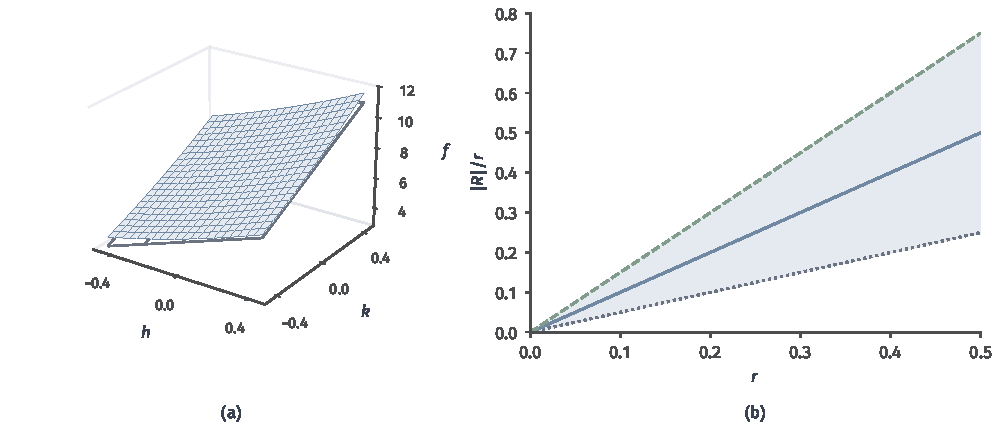
\includegraphics[width=169.0mm]{figures/00-shared/mathematical-preliminaries-upper/00-shared/matplotlib/chapter3-concept-processes/total-differential-remainder.pdf}
 \caption{(a) 二次函数在$(1,2)$附近，灰网格是切平面$P=7+4h+5k$，蓝面是$f(1+h,2+k)$。(b) 令$r=\sqrt{h^2+k^2}$，余项$R=h^2+hk+k^2$满足$r/2\leq R/r\leq3r/2$；阴影给出所有方向的完整范围，三条线是其中的代表值。共同上界随$r\to0$趋零，才保证任意方向都适用同一个线性近似。}
 \label{fig:analysis-process-total-differential-remainder}
\end{figure*}

\paragraph{偏导数连续给出的充分条件}
按定义验证可微需要估计余项，通常不方便。另一种判别只检查偏导数：如果各坐标的变化率在基点附近连续变化，就可以沿坐标逐段走，用它们共同控制全部坐标增量。
与定理~\ref{thm:multivariable-differentiable-necessary}不同，这是一个充分条件，直接保证全微分存在。
\begin{theorem}[偏导数连续与可微性]
\label{thm:multivariable-continuous-partials-sufficient}
设$f:U\to\mathbb R$，$U$开，$\bm a\in U$。若各一阶偏导数在$\bm a$的某个邻域内存在，并在$\bm a$处连续，则$f$在$\bm a$处可微。
\end{theorem}
\begin{proof}
先看$d=2$。从$(a_1,a_2)$走到$(a_1+h_1,a_2+h_2)$，可以先竖直走、再水平走：
\[
 \begin{aligned}
 &f(a_1+h_1,a_2+h_2)-f(a_1,a_2)\\
 &=\bigl[f(a_1+h_1,a_2+h_2)-f(a_1,a_2+h_2)\bigr]\\
 &\quad+\bigl[f(a_1,a_2+h_2)-f(a_1,a_2)\bigr].
 \end{aligned}
\]
第一个方括号只改变第一个坐标，对一元函数$s\mapsto f(s,a_2+h_2)$用中值定理，得到它等于$\partial_1f(\bm\xi_1)h_1$，其中$\bm\xi_1$在这段水平线段上；第二个方括号同理等于$\partial_2f(\bm\xi_2)h_2$，$\bm\xi_2$在竖直线段上。这里用到$\bm h$足够小时两段都在偏导数存在的邻域内。

一般的$d$同样把$\bm a$到$\bm a+\bm h$的增量拆成$d$段，每段只改一个坐标，一元中值定理将第$j$段增量写成$\partial_jf(\bm\xi_j)h_j$，$\bm\xi_j$是第$j$段上的中间点。
减去候选线性项后，误差为$\sum_j\bigl(\partial_jf(\bm\xi_j)-\partial_jf(\bm a)\bigr)h_j$，因此
\[
 \begin{aligned}
 &\left|f(\bm a+\bm h)-f(\bm a)-\sum_{j=1}^d\partial_j f(\bm a)h_j\right|\\
 &\qquad\leq \max_j\left|\partial_j f(\bm\xi_j)-\partial_j f(\bm a)\right|
       \sum_{j=1}^d|h_j|
 =o(\lVert\bm h\rVert_2).
 \end{aligned}
\]
最后一步有两个依据：当$\bm h\to\bm0$时，所有中间点到$\bm a$的距离都不超过$\lVert\bm h\rVert_2$，偏导数在$\bm a$处连续，使最大值一项趋于零；另一方面$\sum_j|h_j|\leq\sqrt d\lVert\bm h\rVert_2$。
这样，各坐标方向上的变化就拼成了同一个有效的全微分。
\end{proof}
偏导数连续只是充分条件：可微只要求函数增量有统一的一阶近似，不要求这些系数随基点连续变化。实际计算中，若各偏导数在所论开集上由连续的表达式给出，就可以直接断定可微。多项式、分母非零的有理函数，以及它们与指数、正弦等连续函数的复合，都属于这种情形。

\paragraph{连续可微函数}
若要求全微分的系数在一个范围内随基点连续变化，就得到连续可微的概念。
实值函数的各一阶偏导数在开集$U$上存在且连续时，称它在$U$上连续可微，记为$C^1(U)$；$C^k(U)$表示直至$k$阶的各偏导数都存在且连续。
定理~\ref{thm:multivariable-continuous-partials-sufficient}保证$C^1$函数处处可微。逆向并不成立，一元函数就足以说明这一点。
\begin{example}[处处可微而导数无界]
\label{ex:multivariable-differentiable-not-c1}
在实轴上令$r(0)=0$，$x\neq0$时令$r(x)=x^2\sin(1/x^2)$。
由于$|r(h)/h|=|h\sin(1/h^2)|\leq|h|\to0$，有$r'(0)=0$；非零点按运算法则求导，得到
\[
 r'(x)=2x\sin(1/x^2)-\frac{2}{x}\cos(1/x^2).
\]
取$x_n=(2\pi n)^{-1/2}$，则$1/x_n^2=2\pi n$，$\sin$项为$0$、$\cos$项为$1$，于是$r'(x_n)=-2/x_n\to-\infty$。所以$r$处处可微，$r'$却在$0$附近无界，在$0$处不连续。
直观上，$r$的振幅被$x^2$压到零，图像在原点与横轴相切；但振荡越来越快，切线斜率剧烈摆动。
在多元情形令$f(\bm x)=r(x_1)$，就得到处处可微而非连续可微的标量函数。
\end{example}

这个例子还说明可微不保证局部Lipschitz连续（定义~\ref{def:ls-lipschitz}）。若$r$在原点的某个邻域内以$L$为Lipschitz常数，该邻域内每个差商的绝对值都不超过$L$，各点导数也就满足$|r'|\leq L$，与$r'(x_n)\to-\infty$矛盾。

\paragraph{必要条件不能反推可微}
可微蕴含连续、偏导数存在和全部双侧方向导数存在。一元函数在一点的导数存在就等价于可微，因为实轴上只有一条直线可走。多元函数还须协调无穷多个输入方向以及弯曲的趋近路径，所以这些必要条件单独或合起来都不能保证可微。下面依次检查它们的逆向。

\paragraph{偏导数存在不保证可微}
坐标偏导数只约束两条坐标切片，并未控制其余方向或路径。
\begin{example}[偏导数存在但不可微]
\label{ex:analysis-partials-not-differentiable}
定义$f:\mathbb{R}^2\to\mathbb{R}$为
\[
 f(x,y)=
 \begin{cases}
  \dfrac{xy}{\sqrt{x^2+y^2}}, & (x,y)\neq(0,0),\\[6pt]
  0, & (x,y)=(0,0).
 \end{cases}
\]
沿两条坐标轴，函数恒为$0$，所以$\partial f/\partial x(0,0)=\partial f/\partial y(0,0)=0$。若$f$在原点可微，由定理~\ref{thm:multivariable-differentiable-necessary}，候选线性部分只能是零映射。可是沿$\bm{h}=(t,t)$，
\[
 \frac{|f(t,t)-f(0,0)|}{\lVert(t,t)\rVert_2}
 =\frac{|t|/\sqrt{2}}{\sqrt{2}|t|}
 =\frac12,
\]
余项与$\lVert\bm{h}\rVert_2$之比不趋于零，故$f$在原点不可微。

用极坐标可以看清曲面的形状：$f=r\cos\theta\sin\theta=\tfrac r2\sin2\theta$。沿每条从原点出发的射线，函数随$r$线性增长，斜率$\tfrac12\sin2\theta$随方向变化。曲面由这些射线组成，像一个起伏的锥面；把它放大任意倍数后形状不变，永远不会变得像一张平面。

沿每个方向$\bm v=(a,b)$，只令$t\downarrow0$的正向方向导数都存在，等于$ab/\sqrt{a^2+b^2}$（零方向取$0$），但它不是关于$\bm v$的线性函数。$t<0$时差商变号，因此$ab\neq0$时双侧方向导数不存在。
最后，由$|xy|/\sqrt{x^2+y^2}\leq\sqrt{x^2+y^2}/2$，$f$在原点连续。
\end{example}

偏导数只看坐标轴，遗漏了其他接近方向；可微则要求曲面放大后接近平面，本例的锥面做不到。本例还说明，即使偏导数存在、全部正向方向导数存在、函数又连续，也推不出可微。这里的正向方向导数是单侧极限，与本节采用的双侧定义不同，使用时要分清。

\paragraph{全部方向导数存在不保证可微}
把坐标切片换成所有固定直线，仍有两件事需要检查：这些变化率能否组成一个线性映射，以及是否有统一的余项控制。先看缺少线性性的情形。
\begin{example}[方向导数不构成线性映射]
\label{ex:multivariable-nonlinear-directional-derivatives}
在非原点处令$p(x,y)=x^3/(x^2+y^2)$，并令$p(0,0)=0$。
沿$\bm v=(a,b)\neq\bm0$，差商为$p(ta,tb)/t=a^3/(a^2+b^2)$，不依赖$t$，所以双侧方向导数存在且$D_{\bm v}p(0,0)=a^3/(a^2+b^2)$。
取坐标方向得到两个偏导数$1$与$0$。若$p$可微，由定理~\ref{thm:multivariable-differentiable-necessary}，沿$(1,1)^\top$的方向导数应为$1\cdot1+0\cdot1=1$，实际却是$1/(1+1)=1/2$。这些方向变化率无法拼成一个线性映射，所以$p$在原点不可微。
\end{example}

示例~\ref{ex:analysis-partials-not-differentiable}只有单侧方向导数；这里的双侧方向导数全部存在，失败只来自线性性。
即使方向导数全部存在并组成一个线性映射，还要检查余项能否统一控制。
\begin{example}[方向导数全为零仍不可微]
\label{ex:multivariable-linear-directionals-not-differentiable}
在非原点处令$q(x,y)=x^3y/(x^4+y^2)$，并令$q(0,0)=0$。
由$2|x^2y|\leq x^4+y^2$，有$|q(x,y)|\leq|x|/2$，故$q$在原点连续。
对固定方向$(a,b)^\top$，若$b\neq0$，
\[
 \frac{q(ta,tb)}t=\frac{t a^3b}{t^2a^4+b^2}\longrightarrow0;
\]
若$b=0$，差商恒为零。因此所有双侧方向导数都为零，它们组成零线性映射。
可是沿$\bm h=(t,t^2)^\top$，$q(t,t^2)=t^5/(2t^4)=t/2$，从而
\[
 \frac{|q(t,t^2)|}{\lVert(t,t^2)\rVert_2}
 =\frac1{2\sqrt{1+t^2}}\longrightarrow\frac12.
\]
候选零映射不满足全微分的余项条件，$q$在原点不可微。
\end{example}

这与示例~\ref{ex:multivariable-parabola-path-limit}中$g$的情形相同：函数沿抛物线有一道坡，每条直线进入原点时都避开了它。方向导数先固定方向再取极限；全微分则要求方向随扰动改变时，误差仍受同一个控制。

\paragraph{连续与偏导数存在互不蕴含}
连续性也推不出微分条件。
例如$f(x,y)=|x|$在整个平面上Lipschitz连续，图像沿$y$轴有一道折痕。原点关于$x$的双侧偏导数不存在，因此$f$在那里不可微。
偏导数存在同样推不出连续：示例~\ref{ex:multivariable-path-limits}中原点置零的$xy/(x^2+y^2)$沿坐标轴恒为零，两个偏导数存在，但它在原点不连续。
所以连续与偏导数存在互不蕴含，可微则同时保证二者。

\paragraph{条件之间的蕴含关系}
把必要条件、充分判别与上面的反例放在一起，得到下面的蕴含链：
\[
 \begin{gathered}
 f\text{在}\bm a\text{的某邻域内连续可微}
 \ \Longrightarrow\ f\text{在}\bm a\text{处可微},\\
 f\text{在}\bm a\text{处可微}
 \ \Longrightarrow\ \text{全部双侧方向导数存在}
 \ \Longrightarrow\ \text{全部偏导数存在}.
 \end{gathered}
\]
第一条由定理~\ref{thm:multivariable-continuous-partials-sufficient}得到，第二条由定理~\ref{thm:multivariable-differentiable-necessary}得到，最后一条只须在全部方向中取坐标方向$\bm e_j$。
同一定理还说明，可微蕴含连续，并且方向导数关于方向是线性映射$\bm v\mapsto\mathrm df_{\bm a}(\bm v)$。
第一行的前提涉及$\bm a$的整个邻域，其余条件只涉及基点$\bm a$本身；链中的方向导数都按双侧极限理解。

各箭头都不能反向：示例~\ref{ex:multivariable-differentiable-not-c1}说明处处可微仍可能不连续可微；示例~\ref{ex:multivariable-nonlinear-directional-derivatives}与示例~\ref{ex:multivariable-linear-directionals-not-differentiable}说明全部双侧方向导数存在仍可能不可微，后者连函数连续、方向导数组成线性映射这两点也都满足；示例~\ref{ex:analysis-partials-not-differentiable}说明偏导数存在不推出全部双侧方向导数存在。不满足偏导数连续这一充分条件时，应回到全微分的定义检查余项。

\subsection{微分的运算法则}
\label{sec:multivariable-differential-rules}

直接按定义求全微分很繁琐。与一元情形一样，可以从简单函数的微分出发，用运算法则组合出复杂函数的微分。
本小节的$f,g$都在同一开集内定义，并在基点$\bm a$处可微，$c$为固定实数。
各法则的证明方法相同：代入各自的一阶展开，整理出关于$\bm h$的线性项，再确认剩下的部分仍是$o(\lVert\bm h\rVert_2)$。这样既证明新函数可微，也读出了它的全微分。

\paragraph{和、差与数乘的微分}
把两个一阶展开相加，
\[
 (f+g)(\bm a+\bm h)=(f+g)(\bm a)+\bigl(\mathrm df_{\bm a}+\mathrm dg_{\bm a}\bigr)(\bm h)+o(\lVert\bm h\rVert_2),
\]
两个线性映射之和仍是线性映射，两个$o(\lVert\bm h\rVert_2)$余项之和仍是$o(\lVert\bm h\rVert_2)$，因此
$\mathrm d(f+g)=\mathrm df+\mathrm dg$。
把加号换成减号，同样的论证给出$\mathrm d(f-g)=\mathrm df-\mathrm dg$。固定系数$c$只会缩放线性项与余项，故$\mathrm d(cf)=c\,\mathrm df$，包括$c=0$的常函数情形。

\paragraph{积的微分}
记$R_f,R_g$为两个一阶展开的余项，都是$o(\lVert\bm h\rVert_2)$。相乘得
\[
 \begin{aligned}
 f(\bm a+\bm h)g(\bm a+\bm h)
 &=\bigl(f(\bm a)+\mathrm df(\bm h)+R_f\bigr)\bigl(g(\bm a)+\mathrm dg(\bm h)+R_g\bigr)\\
 &=f(\bm a)g(\bm a)+g(\bm a)\,\mathrm df(\bm h)+f(\bm a)\,\mathrm dg(\bm h)+(\text{其余各项}).
 \end{aligned}
\]
其余各项要么含有余项$R_f,R_g$乘以有界量，要么是两个线性增量的乘积$\mathrm df(\bm h)\,\mathrm dg(\bm h)=O(\lVert\bm h\rVert_2^2)$，都是$o(\lVert\bm h\rVert_2)$。因此乘积可微，且
\[
 \mathrm d(fg)=g(\bm a)\,\mathrm df+f(\bm a)\,\mathrm dg.
\]
这与一元的$(fg)'=f'g+fg'$形式相同：两个因子各自变化，一阶上贡献可以相加，两个变化同时发生的部分是高阶小量。

\paragraph{商的微分}
设$g(\bm a)\neq0$。可微蕴含连续，所以$g$在$\bm a$附近远离零，$1/g$在$\bm a$附近有定义。记$\delta=g(\bm a+\bm h)-g(\bm a)=\mathrm dg(\bm h)+o(\lVert\bm h\rVert_2)$，它是$O(\lVert\bm h\rVert_2)$。一元函数$1/y$在$g(\bm a)$处的展开给出
\[
 \frac1{g(\bm a)+\delta}=\frac1{g(\bm a)}-\frac{\delta}{g(\bm a)^2}+O(\delta^2).
\]
代入$\delta$的展开，并注意$O(\delta^2)=O(\lVert\bm h\rVert_2^2)$，得到$\mathrm d(1/g)=-\mathrm dg/g(\bm a)^2$。再把$f/g$看成$f\cdot(1/g)$，用积的微分得到
\[
 \mathrm d(f/g)=\frac{g(\bm a)\,\mathrm df-f(\bm a)\,\mathrm dg}{g(\bm a)^2}.
\]
这里分母非零既是定义商函数的条件，也是估计余项的条件。

\paragraph{标量复合函数的微分}
若一元函数$\psi$在$f(\bm a)$处可微，且复合在$\bm a$的邻域内有定义，则$\psi\circ f$在$\bm a$处可微，并且
\[
 \mathrm d(\psi\circ f)=\psi'(f(\bm a))\,\mathrm df.
\]
推导时把内层增量$\delta=f(\bm a+\bm h)-f(\bm a)$代入外层的一元展开$\psi(f(\bm a)+\delta)=\psi(f(\bm a))+\psi'(f(\bm a))\delta+o(|\delta|)$，再把$\delta=\mathrm df(\bm h)+o(\lVert\bm h\rVert_2)$代入。
因为$\delta=O(\lVert\bm h\rVert_2)$，外层余项$o(|\delta|)$仍是$o(\lVert\bm h\rVert_2)$。
例如$-(x^2+y^2)$在$(x,y)$处的全微分为$(h,k)\mapsto-2xh-2yk$，所以$e^{-(x^2+y^2)}$的全微分是$(h,k)\mapsto e^{-(x^2+y^2)}(-2xh-2yk)$：外层只把内层的全微分乘上一个正数。

\paragraph{沿参数曲线的变化率}
外层也可以是多元函数、内层是一元的参数曲线。设$\bm x:I\to U$定义在开区间$I$上，各坐标在$t_0$处可微，记速度向量$\bm x'(t_0)=(x_1'(t_0),\ldots,x_d'(t_0))^\top$；又设$f$在$\bm a=\bm x(t_0)$处可微。则$t\mapsto f(\bm x(t))$在$t_0$处可微，且
\begin{equation}
 \frac{\mathrm d}{\mathrm dt}f(\bm x(t))\Big|_{t=t_0}
 =\mathrm df_{\bm a}\bigl(\bm x'(t_0)\bigr)
 =\sum_{j=1}^d\partial_jf(\bm a)\,x_j'(t_0).
\label{eq:multivariable-curve-chain-rule}
\end{equation}
推导与上一段相同。记内层增量$\bm k=\bm x(t_0+s)-\bm x(t_0)$，各坐标的一元展开给出$\bm k=s\bm x'(t_0)+o(|s|)$，因而$\lVert\bm k\rVert_2=O(|s|)$。代入$f$的一阶展开，
\[
 f(\bm x(t_0+s))-f(\bm a)=\mathrm df_{\bm a}(\bm k)+o(\lVert\bm k\rVert_2)
 =s\,\mathrm df_{\bm a}(\bm x'(t_0))+o(|s|),
\]
第二步用了全微分的线性，以及线性映射把长度为$o(|s|)$的向量仍变成$o(|s|)$的数。除以$s$并令$s\to0$即得。
内层的变化先在输入空间中产生速度向量$\bm x'(t_0)$，外层的全微分再作用于这个方向。取直线$\bm x(t)=\bm a+t\bm v$，便回到方向导数公式$D_{\bm v}f(\bm a)=\mathrm df_{\bm a}(\bm v)$。下一小节用式~\eqref{eq:multivariable-curve-chain-rule}说明梯度与等值曲线的切向正交；一般向量值映射的复合在第~\ref{sec:analysis-vector-chain-matrix-calculus}节处理。

\paragraph{二次型的微分}
二次型是向量自变量的标量函数，平方误差、能量函数等都含有这种结构。考虑$q(\bm{x})=\bm{x}^{\top}\bm{A}\bm{x}=\sum_{i,j}A_{i,j}x_ix_j$，其中$\bm{A}\in\mathbb{R}^{d\times d}$固定。它是有限个乘积的和，可以直接用乘积法则：把两个$\bm x$看成两个因子，每次只让一个变化，
\begin{align*}
  \mathrm{d}q_{\bm x}(\bm h)
  &=
  \bm h^{\top}\bm{A}\bm{x}
  +\bm{x}^{\top}\bm{A}\bm h\\
  &=
  \bm{x}^{\top}(\bm{A}^{\top}+\bm{A})\bm h.
\end{align*}
第二步用到$\bm h^\top\bm A\bm x$是一个实数，等于自己的转置$\bm x^\top\bm A^\top\bm h$。所以全微分的系数，即各偏导数排成的列向量，为
\begin{equation}
  \bigl(\partial_1q(\bm x),\ldots,\partial_dq(\bm x)\bigr)^\top
  =
  (\bm{A}+\bm{A}^{\top})\bm{x}.
\label{eq:analysis-quadratic-form-gradient}
\end{equation}
当$\bm{A}$对称时，式~\eqref{eq:analysis-quadratic-form-gradient}化为$2\bm{A}\bm{x}$，与一元的$(ax^2)'=2ax$对应。$\bm A$不对称时不能写成$2\bm{A}\bm{x}$，否则就默认了对称性。
例如
\[
 \bm A=\begin{bmatrix}0&1\\0&0\end{bmatrix}
\]
时$q=x_1x_2$，直接求偏导得$(x_2,x_1)^\top$，与$(\bm A+\bm A^\top)\bm x$一致；而$2\bm A\bm x=(2x_2,0)^\top$是错的。

\paragraph{二次型的精确增量}
乘积法则只给出一阶项。对二次型还可以直接写出完整增量，把一阶项与实际误差放在同一个式子里。设$\bm S$对称，展开得
\[
 q(\bm x+\bm h)-q(\bm x)
 =\bm h^\top\bm S\bm x+\bm x^\top\bm S\bm h+\bm h^\top\bm S\bm h
 =2\bm x^\top\bm S\bm h+\bm h^\top\bm S\bm h,
\]
其中用到$\bm h^\top\bm S\bm x=(\bm h^\top\bm S\bm x)^\top=\bm x^\top\bm S\bm h$。由Cauchy--Schwarz不等式与谱范数的定义（第~\ref{sec:multivariable-operator-norm}节），
\[
 |\bm h^\top\bm S\bm h|\leq\lVert\bm h\rVert_2\lVert\bm S\bm h\rVert_2\leq\lVert\bm S\rVert_2\lVert\bm h\rVert_2^2 .
\]
所以余项不只是$o(\lVert\bm h\rVert_2)$，而是被一个明确的二次量控制；这也独立地证明了$q$可微，且$\mathrm dq_{\bm x}(\bm h)=2\bm x^\top\bm S\bm h$。
例如$x^2+xy+y^2=\bm x^\top\bm S\bm x$，其中
\[
 \bm S=\begin{bmatrix}1&1/2\\1/2&1\end{bmatrix}
\]
的特征值为$3/2$与$1/2$。对称矩阵的谱范数是特征值绝对值的最大者（第~\ref{chap:eigen-spectral-decomposition}章），故$\lVert\bm S\rVert_2=3/2$，这正是示例~\ref{ex:multivariable-quadratic-differential}中余项上界$\tfrac32(h^2+k^2)$的常数。
二次项$\bm h^\top\bm S\bm h$在第~\ref{sec:multivariable-curvature-error}节成为Hessian二次型，梯度和余项估计也将复用这个例子。

\subsection{梯度与内积}
\label{sec:multivariable-gradient-inner-product}

可微时，全微分$\mathrm df_{\bm a}$是$\mathbb R^d$上的线性泛函，即对偶空间中的元素（第~\ref{sec:ls-dual-spaces}节）：它读取一个输入扰动，给出函数值的一阶变化。泛函本身不是输入空间中的向量，不能画成地图上的箭头。第~\ref{sec:ls-riesz-representation}节的Riesz表示定理说明，选定内积后，每个线性泛函都等于与唯一一个向量的内积。把这个向量作为全微分的表示，就得到梯度。
\begin{definition}[梯度]
\label{def:multivariable-gradient}
设$\mathbb R^d$上取定内积$\langle\cdot,\cdot\rangle$，$f:U\to\mathbb R$在$\bm a$处可微。满足
\[
 \mathrm df_{\bm a}(\bm h)=\langle\nabla f(\bm a),\bm h\rangle\qquad(\bm h\in\mathbb R^d)
\]
的唯一向量$\nabla f(\bm a)\in\mathbb R^d$称为$f$在$\bm a$处的\term{梯度}（gradient）。未加说明时取标准欧氏内积$\langle\bm x,\bm y\rangle=\bm x^\top\bm y$。
\end{definition}
在标准欧氏内积下，比较定理~\ref{thm:multivariable-differentiable-necessary}中的$\mathrm df_{\bm a}(\bm h)=\sum_j\partial_jf(\bm a)h_j$与$\nabla f(\bm a)^\top\bm h$，逐个取$\bm h=\bm e_j$，得到
\begin{equation}
 \nabla f(\bm a)=\bigl(\partial_1f(\bm a),\ldots,\partial_df(\bm a)\bigr)^\top .
\label{eq:multivariable-gradient-coordinates}
\end{equation}
于是可微函数满足$f(\bm a+\bm h)=f(\bm a)+\nabla f(\bm a)^\top\bm h+o(\lVert\bm h\rVert_2)$，方向导数为$D_{\bm v}f(\bm a)=\nabla f(\bm a)^\top\bm v$。
例如$f(x,y)=x^2+xy+y^2$的梯度为$\nabla f(x,y)=(2x+y,x+2y)^\top$，$\nabla f(1,2)=(4,5)^\top$；由式~\eqref{eq:analysis-quadratic-form-gradient}，一般二次型有$\nabla_{\bm x}(\bm x^\top\bm A\bm x)=(\bm A+\bm A^\top)\bm x$。
梯度与输入属于同一个空间：$(4,5)^\top$可以画成地图平面上从$(1,2)$出发的一支箭头，而不是曲面上的向量。

若$f$在开集$U$上处处可微，把每一点的梯度放在该点，就得到$U$上的向量场$\nabla f:U\to\mathbb R^d$，称为$f$的梯度场。例如第~\ref{sec:multivariable-scalar-fields}节的标量场$x^2+y^2$的梯度场是$(2x,2y)^\top$，箭头从原点向外，离原点越远越长，与那里观察到的“等值圆越来越密”相符。哪些向量场是某个标量场的梯度场，留到第~\ref{sec:multivariable-potential-path-independence}节研究。

表示向量随泛函线性变化，所以上一小节的法则直接改写为梯度的法则：$\nabla(f\pm g)=\nabla f\pm\nabla g$，$\nabla(cf)=c\nabla f$，$\nabla(fg)=g(\bm a)\nabla f+f(\bm a)\nabla g$，$\nabla(\psi\circ f)=\psi'(f(\bm a))\nabla f$。例如$\nabla e^{-(x^2+y^2)}=e^{-(x^2+y^2)}(-2x,-2y)^\top$，与$-(x^2+y^2)$的梯度同向，都指向原点。

\paragraph{偏导数向量与梯度}
式~\eqref{eq:multivariable-gradient-coordinates}的右侧在偏导数全部存在时就能写出，本书在这种情形下也用记号$\nabla f(\bm a)$表示这一列偏导数。但第~\ref{sec:multivariable-total-differentiation}节的反例说明，这时它只是坐标变化率排成的向量：示例~\ref{ex:multivariable-nonlinear-directional-derivatives}中这一列是$(1,0)^\top$，却给不出沿$(1,1)^\top$的方向导数。只有确认可微以后，它才代表对所有方向同时有效的一阶近似，才可以用内积计算任意方向导数，并解释为最快上升的方向。

梯度的列向量排列也来自所选内积和坐标：全微分本身是一个线性作用，标准欧氏内积把它的系数原样排成列向量。换用其他内积时，同一个全微分由另一个向量表示。

\paragraph{改变内积时的梯度}
设$\mathbb R^d$上的内积在标准坐标下写成$\langle\bm x,\bm y\rangle_{\bm G}=\bm x^\top\bm G\bm y$，其中$\bm G$对称正定。第~\ref{sec:ls-gram-coordinates}节说明，任何内积在坐标下都是这种形式，$\bm G$就是基的Gram矩阵。记全微分的系数向量为$\bm c=\bigl(\partial_jf(\bm a)\bigr)_{j=1}^d$。要求$\mathrm df_{\bm a}(\bm h)=\bm c^\top\bm h=\bm g^\top\bm G\bm h$对所有$\bm h$成立，等价于$\bm G\bm g=\bm c$，所以
\begin{equation}
 \nabla_{\bm G}f(\bm a)=\bm G^{-1}\bigl(\partial_jf(\bm a)\bigr)_{j=1}^d .
\label{eq:multivariable-gradient-gram}
\end{equation}
系数向量$\bm c$由函数本身决定；改变的只是用哪个向量来表示同一个全微分。
\begin{example}[加权内积下的梯度]
\label{ex:multivariable-weighted-gradient}
仍取$f(x,y)=x^2+xy+y^2$与基点$(1,2)$，系数向量为$(4,5)^\top$。改用$\bm G=\operatorname{diag}(4,1)$给出的加权内积$\langle\bm x,\bm y\rangle_{\bm G}=4x_1y_1+x_2y_2$，由式~\eqref{eq:multivariable-gradient-gram}，
\[
 \nabla_{\bm G}f(1,2)=\operatorname{diag}(1/4,1)\,(4,5)^\top=(1,5)^\top.
\]
核对：$\langle(1,5)^\top,(h,k)^\top\rangle_{\bm G}=4h+5k$，正是同一个全微分。欧氏梯度$(4,5)^\top$与加权梯度$(1,5)^\top$方向不同：加权长度把第一坐标的位移计为原来的两倍，沿它走同样的加权距离只需更小的坐标位移。
\end{example}
这与第~\ref{sec:ls-riesz-representation}节的结论一致：读取本身不变，表示向量随内积改变。

\paragraph{最陡上升方向}
设$f$在$\bm a$处可微，$\bm u$满足$\lVert\bm u\rVert=1$，这里的长度由所选内积诱导。由Cauchy--Schwarz不等式（定理~\ref{thm:linear-algebra-cauchy-schwarz}），
\[
 D_{\bm u}f(\bm a)=\langle\nabla f(\bm a),\bm u\rangle\leq\lVert\nabla f(\bm a)\rVert.
\]
梯度非零时，取$\bm u=\nabla f(\bm a)/\lVert\nabla f(\bm a)\rVert$即达到等号。所以在所选内积的单位长度约束下，梯度方向是局部上升最快的方向，最大坡度等于梯度的长度；反方向$-\nabla f(\bm a)$则下降最快。
示例~\ref{ex:multivariable-weighted-gradient}中，欧氏单位长度下最快方向沿$(4,5)^\top$，加权单位长度下则沿$(1,5)^\top$。“最快”总是相对某种长度而言的。

\paragraph{梯度与等值曲线}
若$\bm u$与梯度正交，方向导数为零，函数值一阶上不变。设$\bm x:I\to U$是一条落在等值集$\{\bm y:f(\bm y)=f(\bm a)\}$中的可微曲线，$\bm x(t_0)=\bm a$。$f(\bm x(t))$恒为常数，由式~\eqref{eq:multivariable-curve-chain-rule}，
\[
 0=\frac{\mathrm d}{\mathrm dt}f(\bm x(t))\Big|_{t=t_0}=\langle\nabla f(\bm a),\bm x'(t_0)\rangle,
\]
所以梯度与这条曲线的切向量正交。这里假定了等值集中确有经过$\bm a$的可微曲线；整个等值集在$\bm a$附近是否为光滑曲线或曲面，还需要第~\ref{sec:analysis-implicit-parameter-integral}章的隐函数定理及梯度非零这一非退化条件。梯度为零只说明一阶项消失，函数在该点附近怎样变化，要由第~\ref{sec:multivariable-curvature-error}节的高阶微分继续判断。

图~\ref{fig:analysis-process-gradient-level-curves}用同一个二次函数比较梯度方向、等值曲线切向及另一个单位方向。
\begin{figure}[!htbp]
 \centering
 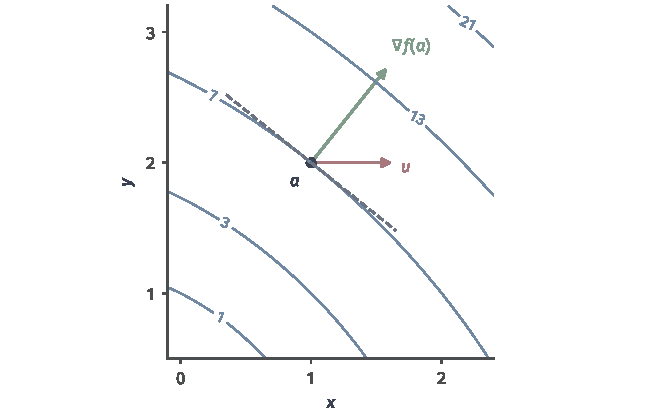
\includegraphics[width=112.0mm]{figures/00-shared/mathematical-preliminaries-upper/00-shared/matplotlib/chapter3-concept-processes/gradient-level-curves.pdf}
 \caption{$f=x^2+xy+y^2$的等值曲线，标注为函数值；基点$a=(1,2)$处$\nabla f=(4,5)^\top$，图中绿箭头按$0.15$倍绘制。灰虚线沿$(5,-4)^\top$，与梯度垂直，因而与经过$a$的等值曲线相切；红箭头为$u=(1,0)^\top$。比较最快上升方向时须先归一化，不能直接比较图中箭头长度。}
 \label{fig:analysis-process-gradient-level-curves}
\end{figure}

\subsection{中值估计与局部Lipschitz性}
\label{sec:multivariable-scalar-mean-value-lipschitz}

微分描述一点附近的变化。要估计两点之间的有限变化，可以沿连接两点的线段把函数限制为一元函数，再使用一元中值定理。前提是整条线段都在定义域内。
记$[\bm x,\bm y]=\{\bm x+t(\bm y-\bm x):0\leq t\leq1\}$为连接两点的线段。
\begin{theorem}[多元标量函数的中值公式]
\label{thm:multivariable-scalar-mean-value}
设$f$在包含$[\bm x,\bm y]$的开集上可微，$\bm x\neq\bm y$。则存在$\theta\in(0,1)$使
\[
 f(\bm y)-f(\bm x)=\nabla f(\bm x+\theta(\bm y-\bm x))^\top(\bm y-\bm x).
\]
\end{theorem}
\begin{proof}
令$\phi(t)=f(\bm x+t(\bm y-\bm x))$，$t\in[0,1]$，它是$f$在线段上的一元切片。$\phi'(t)$就是$f$在点$\bm x+t(\bm y-\bm x)$处沿$\bm y-\bm x$的方向导数，所以$\phi'(t)=\nabla f(\bm x+t(\bm y-\bm x))^\top(\bm y-\bm x)$。
对$\phi$在$[0,1]$上使用一元中值定理，$\phi(1)-\phi(0)=\phi'(\theta)$，这就是所述等式。
\end{proof}
等式说明，两点之间的平均变化率等于线段上某一点沿该方向的瞬时变化率。这是一元“平均斜率等于某点切线斜率”的直接推广。
例如$f(x,y)=x^2+y^2$，$\bm x=(0,0)$、$\bm y=(1,1)$，左侧为$2$；右侧为$\nabla f(\theta,\theta)^\top(1,1)^\top=4\theta$，取$\theta=1/2$即相等，中值点恰为线段中点。

\paragraph{局部Lipschitz性}
\phantomsection
\label{def:multivariable-lipschitz}
定义~\ref{def:ls-lipschitz}已经给出Lipschitz连续与局部Lipschitz连续：存在常数$L$，使输出距离不超过输入距离的$L$倍，局部情形允许常数随邻域改变。那里只说明了这种误差控制的含义，本小节的新任务是由导数求出这样的常数。

中值公式把有限增量写成某点梯度与位移的内积；若梯度的长度有统一上界，就能用输入距离的常数倍控制输出变化。以下距离都取欧氏范数。优化中常用这种控制由步长估计函数值的变化。

先看两个不依赖导数就能读出常数的例子。线性函数$f(\bm x)=\bm a^\top\bm x$满足$|f(\bm x)-f(\bm y)|=|\bm a^\top(\bm x-\bm y)|\leq\lVert\bm a\rVert_2\lVert\bm x-\bm y\rVert_2$，Lipschitz常数可取$\lVert\bm a\rVert_2$，它恰是梯度的长度。
欧氏范数$f(\bm x)=\lVert\bm x\rVert_2$由三角不等式满足$|\lVert\bm x\rVert_2-\lVert\bm y\rVert_2|\leq\lVert\bm x-\bm y\rVert_2$，常数为$1$，尽管它在原点不可微。所以Lipschitz连续本身不要求处处可微。

要把梯度界转化为Lipschitz常数，两点之间的线段必须留在定义域内。若集合$D$中任意两点之间的线段都含于$D$，就称$D$为凸集。在凸开集上，梯度长度的统一上界恰好就是Lipschitz常数。
\begin{theorem}[梯度有界与Lipschitz条件]
\label{thm:multivariable-gradient-lipschitz}
设$U\subseteq\mathbb R^d$为凸开集，$f:U\to\mathbb R$可微。则$f$在$U$上以$L$为Lipschitz常数，当且仅当$\lVert\nabla f(\bm x)\rVert_2\leq L$对所有$\bm x\in U$成立。
\end{theorem}
\begin{proof}
若梯度长度不超过$L$，任取$\bm x\neq\bm y$，凸性保证线段$[\bm x,\bm y]\subseteq U$。由中值公式与内积不等式，
\[
 |f(\bm y)-f(\bm x)|=\bigl|\nabla f(\bm\xi)^\top(\bm y-\bm x)\bigr|\leq\lVert\nabla f(\bm\xi)\rVert_2\lVert\bm y-\bm x\rVert_2\leq L\lVert\bm y-\bm x\rVert_2.
\]
反过来，设$f$以$L$为Lipschitz常数。固定$\bm x$，若$\nabla f(\bm x)\neq\bm0$，取单位方向$\bm u=\nabla f(\bm x)/\lVert\nabla f(\bm x)\rVert_2$，则
\[
 \lVert\nabla f(\bm x)\rVert_2=D_{\bm u}f(\bm x)=\lim_{t\downarrow0}\frac{f(\bm x+t\bm u)-f(\bm x)}t\leq\lim_{t\downarrow0}\frac{Lt}t=L.
\]
梯度为零时不等式自然成立。
\end{proof}
几何上，若坡度处处不超过$L$，沿直线走过距离$\rho$，高度最多改变$L\rho$；反过来，Lipschitz常数也限制了每一点最陡方向的坡度。
例如$f(x,y)=\sin x+\cos y$满足$\lVert\nabla f\rVert_2=\sqrt{\cos^2x+\sin^2y}\leq\sqrt2$，所以它在整个平面上以$\sqrt2$为Lipschitz常数。

定理中的凸性不能省略。在不凸的区域上，梯度可以处处很小，函数值却在两个很近的点之间相差很大。
\begin{example}[非凸区域上梯度有界而不Lipschitz]
\label{ex:multivariable-nonconvex-lipschitz-failure}
取去掉负$x$轴的环形区域$D=\{1<\lVert\bm x\rVert_2<2\}\setminus\{(x,0):x<0\}$，令$f(\bm x)$为点$\bm x$的极角，取值于$(-\pi,\pi)$。$f$在$D$上可微，$\lVert\nabla f\rVert_2=1/r<1$，坡度处处小于$1$。
但取负$x$轴两侧的点$(-1.5,\pm\varepsilon)$，两点距离为$2\varepsilon$，极角却分别接近$\pi$与$-\pi$，相差接近$2\pi$。令$\varepsilon\to0$，函数值之差与距离之比无界，所以$f$在$D$上不是Lipschitz函数。
\end{example}

连接这两点的直线段穿过被去掉的负$x$轴，不在$D$内，中值公式无法使用。$D$内连接两点的路径必须绕过原点，长度远大于$2\varepsilon$。可见梯度界只能沿含于定义域的线段转化为函数值之差的界。

局部情形不需要整个定义域凸。若$f\in C^1(U)$，在每个基点附近取一个包含在$U$内的闭球。连续函数$\lVert\nabla f\rVert_2$在这个闭有界集上有界（定理~\ref{thm:multivariable-extreme-value}），因而在同心的开球上也有界。开球是凸开集，由定理~\ref{thm:multivariable-gradient-lipschitz}，$f$在这个开球上Lipschitz连续，所以$f$局部Lipschitz连续。
各点的局部常数不一定有共同上界：$f(x,y)=x^2$连续可微，但$\lVert\nabla f\rVert_2=2|x|$在全平面无界，因而它不是全域Lipschitz函数。

\paragraph{三种控制的强弱}
至此出现了三种关于函数变化的结论，强度各不相同。连续只保证$\bm x\to\bm a$时$f(\bm x)\to f(\bm a)$，不给出趋近的速度。可微给出渐近的线性近似：误差是$o(\lVert\bm h\rVert_2)$，但对一个给定的有限步长，它不说明误差有多大。梯度的统一界则沿含于定义域的线段控制有限距离上的变化，常数明确，却只估计变化的大小，不估计线性预测还差多少。

要估计一阶预测还差多少，需要把后两种结论结合起来，考察导数本身沿线段怎样变化。第~\ref{sec:multivariable-curvature-error}节的Taylor公式用二阶导数描述这种变化；只用一阶导数的余项界，以及误差被放大多少倍的局部条件数，集中在第~\ref{chap:differential-perturbation-analysis}章讨论。

\section{多元向量值函数的微分}
\label{sec:multivariable-vector-differentiation}

前面每个输入只产生一个实数。本节研究同时产生$m$个输出分量的映射$F:U\subseteq\mathbb R^d\to\mathbb R^m$，关心输入稍作改变时输出点整体怎样移动。

例如极坐标映射$(r,\theta)\mapsto(r\cos\theta,r\sin\theta)$把两个参数变成平面上的点，神经网络的一层把输入向量变成另一个向量；参数曲线（$d=1$）与参数曲面（$d=2$、$m=3$）也是这种映射。
输出只有有限个分量，所以可以逐个分量使用前面的结论。但每个分量仍要对全部输入方向整体扰动，不能用坐标切片代替各分量的全微分。本节先用一个线性映射定义整体可微并引入Jacobian矩阵，再给出复合映射的导数，最后用导数的算子范数估计有限增量。

\subsection{Jacobian矩阵}

向量值函数由它的全部输出分量确定，因此按分量书写。
\begin{definition}[多元向量值函数]
\label{def:multivariable-vector-function}
映射$F:U\subseteq\mathbb R^d\to\mathbb R^m$称为多元向量值函数，写作$F=(F_1,\ldots,F_m)^\top$，其中每个$F_i:U\to\mathbb R$为多元标量函数。
\end{definition}
向量值函数的极限与连续性已在第~\ref{sec:multivariable-joint-limit-section}节与第~\ref{sec:multivariable-continuity}节定义，第~\ref{sec:multivariable-field-limits-continuity}节回顾了要点：输出点整体接近，等价于每个输出分量接近；每个分量的极限仍是对全部输入方向的联合极限。本节在连续性的基础上进一步研究线性近似。向量场是$m=d$的特例，下面的结论对它同样适用。

\paragraph{微分与Jacobian矩阵}

标量输出的全微分是到实数的线性映射，也称线性泛函。向量输出的全微分则要把输入扰动映射为$m$维输出扰动。
有限维线性映射由矩阵表示，矩阵的每一行记录一个输出分量的系数。
\begin{definition}[向量值函数的微分]
\label{def:multivariable-vector-differential}
设$U$开，$F:U\to\mathbb R^m$，$\bm a\in U$。若存在线性映射$\mathrm dF_{\bm a}:\mathbb R^d\to\mathbb R^m$，记它在标准基下的矩阵为$\bm J_F(\bm a)\in\mathbb R^{m\times d}$，使
\begin{equation}
 F(\bm a+\bm h)=F(\bm a)+\bm J_F(\bm a)\bm h+o(\lVert\bm h\rVert_2),
\label{eq:analysis-jacobian-linearization}
\end{equation}
则称$F$在$\bm a$处可微，余项按输出欧氏范数理解。
$\mathrm dF_{\bm a}(\bm h)=\bm J_F(\bm a)\bm h$称为$F$在$\bm a$处的微分，矩阵$\bm J_F(\bm a)$称为\term{Jacobian矩阵}（Jacobian matrix）。
\end{definition}
向量值函数可微当且仅当每个输出分量$F_i$可微。正向只需从向量余项取第$i$个分量，它的绝对值不超过向量余项的欧氏长度，于是得到$F_i$的标量展开；反向则把有限个分量的$o(\lVert\bm h\rVert_2)$余项用欧氏范数合并，合并后仍是$o(\lVert\bm h\rVert_2)$。
由此，Jacobian的第$i$行是分量梯度的转置$\nabla F_i^\top$，第$i,j$个元素为$\partial_jF_i$；微分若存在则唯一。$C^k$向量值函数指所有输出分量都属于$C^k$。

本书把输入、输出都写成列向量，因此$\bm J_F(\bm a)$是“输出维数$\times$输入维数”的矩阵：第$i$行记录第$i$个输出对各输入的偏导数，$\bm J_F(\bm a)\bm h$的形状为$(m\times d)(d\times1)=m\times1$，与输出一致。$m=1$时Jacobian是$1\times d$的行向量$\nabla f(\bm a)^\top$，梯度则是列向量，二者互为转置。

\paragraph{Jacobian矩阵的几何意义}
按行看，Jacobian记录各输出分量的梯度；按列看，它记录各输入坐标对输出点的推动。第$j$列
\[
 \bm J_F(\bm a)\bm e_j=(\partial_jF_1,\ldots,\partial_jF_m)^\top
\]
表示：只把第$j$个输入增加一个很小的量$t$时，输出点大约移动这个向量的$t$倍。一般扰动$\bm h=\sum_jh_j\bm e_j$的一阶效果，就是这些列按$h_j$加权求和。
对$d=m=2$，由此得到局部伸缩的图像。以$\bm a$为角、边长为$\varepsilon$的小正方形由$\varepsilon\bm e_1,\varepsilon\bm e_2$张成，它的像近似是由$\varepsilon\bm J_F\bm e_1,\varepsilon\bm J_F\bm e_2$张成的平行四边形。行列式的绝对值是线性映射对面积的缩放倍数（第~\ref{sec:prelim-determinants}节），所以像的面积约为$|\det\bm J_F(\bm a)|\varepsilon^2$；行列式的符号说明局部是否翻转了定向。

极坐标映射是这种局部伸缩的一个具体例子。
\begin{example}[极坐标映射的Jacobian矩阵]
\label{ex:multivariable-polar-jacobian}
考虑极坐标映射
\[
 P(r,\theta)=(r\cos\theta,r\sin\theta)^\top.
\]
逐个输出分量求偏导，得到
\[
\begin{gathered}
\bm J_P(r,\theta)=\begin{bmatrix}\cos\theta&-r\sin\theta\\ \sin\theta&r\cos\theta\end{bmatrix}\\
\det\bm J_P=r\cos^2\theta+r\sin^2\theta=r.
\end{gathered}
\]
第一列是单位径向向量：$r$增加$\mathrm dr$，点沿射线向外移动$\mathrm dr$。第二列长度为$r$、沿圆周切向：$\theta$增加$\mathrm d\theta$，点沿半径为$r$的圆移动约$r\,\mathrm d\theta$。因此参数平面中面积为$\mathrm dr\,\mathrm d\theta$的小矩形，变成面积约为$r\,\mathrm dr\,\mathrm d\theta$的小扇形块。
\end{example}

离原点越远，同样的角度增量扫过的弧越长，面积放大越多。第~\ref{sec:classical-change-variables}节的区域积分换元就用这个倍数校正面积。

对一般的非线性映射，小网格块的像是弯边块，线性近似把它换成平行四边形。图~\ref{fig:analysis-process-jacobian-grid-cell}画出了这种对应。图中$\det J_T(a)=1\times0.6-0.25\times0.3=0.525$，所以绿色小方块的像面积约为原面积的一半。
\begin{figure*}[!htbp]
 \centering
 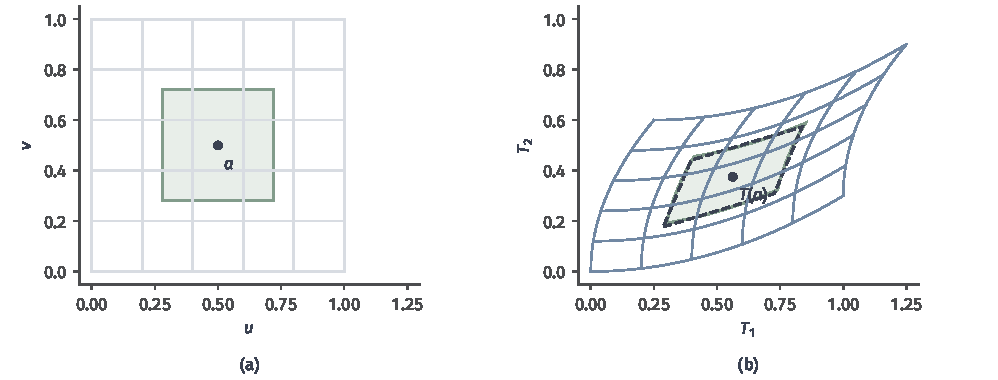
\includegraphics[width=169.0mm]{figures/00-shared/mathematical-preliminaries-upper/00-shared/matplotlib/chapter3-concept-processes/jacobian-grid-cell.pdf}
 \caption{取$T(u,v)=(u+v^2/4,\,0.6v+0.3u^2)$，$a=(0.5,0.5)$。(a) 输入网格及绿色小方块。(b) 非线性像为弯边块，黑虚线为$T(a)+J_T(a)(h,k)^\top$给出的平行四边形；$J_T(a)=\bigl[\begin{smallmatrix}1&0.25\\0.3&0.6\end{smallmatrix}\bigr]$。有限块不与线性像完全重合，缩小扰动后才由可微余项控制差异。}
 \label{fig:analysis-process-jacobian-grid-cell}
\end{figure*}

输入、输出维数不同时，同一个原则给出非方阵的Jacobian。
\begin{example}[空间螺旋线的Jacobian矩阵]
\label{ex:multivariable-helix-jacobian}
令$\bm\gamma(t)=(\cos t,\sin t,t)^\top$，$t\in\mathbb R$，输入一维、输出三维。逐分量求导得
\[
 \bm J_{\bm\gamma}(t)=\begin{bmatrix}-\sin t\\ \cos t\\ 1\end{bmatrix}\in\mathbb R^{3\times1}.
\]
它把参数增量$s$映为$s\bm J_{\bm\gamma}(t)$：点沿速度向量$\bm\gamma'(t)$移动。这一列就是曲线的切向量，长度为$\sqrt2$，说明参数每增加一个单位，点约移动$\sqrt2$的距离。
\end{example}
螺旋线的Jacobian不是方阵，没有行列式可言，局部伸缩由切向量的长度描述。极坐标与螺旋线说明，“微分是线性映射”这一原则在不同输入、输出维数下给出形状不同的矩阵，不能默认Jacobian是方阵或有行列式。梯度映射$\bm x\mapsto\nabla f(\bm x)$本身也是从$\mathbb R^d$到$\mathbb R^d$的向量值映射，第~\ref{sec:multivariable-curvature-error}节将研究它的微分，并由此得到Hessian矩阵。

\paragraph{Jacobian矩阵的计算}
计算Jacobian矩阵时，先把每个输出分量当作标量函数求偏导，再按行排列；排好后核对矩阵形状是否为“输出维数$\times$输入维数”。
例如$F(x,y)=(x^2+xy,y^2)^\top$的Jacobian为
\[
 \bm J_F(x,y)=\begin{bmatrix}2x+y&x\\0&2y\end{bmatrix}.
\]
在$(1,2)$处，它把扰动$(h,k)^\top$的一阶影响写成$(4h+k,4k)^\top$。第一行说明第一个输出同时受两个输入推动，第二行说明第二个输出只随$y$变化；两列分别记录沿$x$、沿$y$移动时输出点的位移方向。

再看机器学习中常用的一个向量值映射。它把任意一组实数变成总和为$1$的正权重：先取指数，再除以共同的总和。
这就是$n$维\term{归一化指数映射}（softmax），分类模型常用它把各类别的得分变成概率。对正整数$n$和
$\bm{z}\in\mathbb{R}^n$，令
\[
 \begin{gathered}
s_i(\bm{z})
  =
  \frac{e^{z_i}}{\sum_{k=1}^n e^{z_k}}\\
i=1,\ldots,n.
 \end{gathered}
\]
记分母为$Z=\sum_k e^{z_k}$，它对$z_j$的偏导数为$e^{z_j}$。对分子$e^{z_i}$求偏导，$i=j$时得$e^{z_i}$，$i\neq j$时得$0$，记为$\mathbb{I}\{i=j\}e^{z_i}$。商法则给出
\[
  \frac{\partial s_i}{\partial z_j}
  =
  \frac{\mathbb{I}\{i=j\}e^{z_i}Z-e^{z_i}e^{z_j}}{Z^2}
  =
  s_i\bigl(\mathbb{I}\{i=j\}-s_j\bigr).
\]
因此整个Jacobian矩阵为
\begin{equation}
  \bm{J}_{\bm{s}}(\bm{z})
  =
  \operatorname{diag}(\bm{s})-\bm{s}\bm{s}^{\top}.
\label{eq:analysis-softmax-jacobian}
\end{equation}
这里$\operatorname{diag}(\bm s)$表示以$s_1,\ldots,s_n$为对角元、其他元素为零的对角矩阵。

当$n\geq2$时，对角项$s_i(1-s_i)$为正，描述提高$z_i$对自身分量的影响。非对角项$-s_is_j$为负，它来自共同分母：提高一个得分会压低其余分量。当$n=1$时输出恒为$1$，Jacobian为零。

每行元素之和为$s_i-s_i\sum_js_j=0$。这与给所有$z_i$加同一常数不改变输出相符：沿方向$(1,\ldots,1)^\top$的一阶变化为零。

在最简单的情形中，可以用数值核对式~\eqref{eq:analysis-softmax-jacobian}给出的线性近似。
\begin{example}[二维softmax的Jacobian矩阵]
\label{ex:multivariable-softmax-jacobian-check}
取$n=2$、$\bm z=\bm 0$，则$\bm s=(1/2,1/2)^\top$，由式~\eqref{eq:analysis-softmax-jacobian}，
\[
 \bm J_{\bm s}(\bm 0)
 =\begin{bmatrix}1/2&0\\0&1/2\end{bmatrix}-\begin{bmatrix}1/4&1/4\\1/4&1/4\end{bmatrix}
 =\begin{bmatrix}1/4&-1/4\\-1/4&1/4\end{bmatrix}.
\]
把$z_1$提高$0.1$，线性近似给出$\bm s$的增量约为
\[
 \bm J_{\bm s}(\bm 0)(0.1,0)^\top=(0.025,-0.025)^\top,
\]
即$s_1\approx0.525$、$s_2\approx0.475$。实际值为$s_1=e^{0.1}/(e^{0.1}+1)\approx0.52498$、$s_2\approx0.47502$。
\end{example}

线性近似与实际值只差约$2\times10^{-5}$，远小于输入改变量$0.1$；两个分量的增量一正一负、总和为零，与$s_1+s_2$恒为$1$相符。

\subsection{微分的运算法则}
\label{sec:analysis-vector-chain-matrix-calculus}

与标量情形一样，复杂映射的Jacobian可以由简单映射的Jacobian组合得到。各法则以运算有定义为前提：输出形状相同的向量值函数可以相加、相减，任何向量值函数都可以数乘；复合则要求前一映射的输出落在后一映射的定义域内。
两个向量之间的乘法需要先指定含义；下面先处理线性运算与复合，再用链式法则处理内积等乘法结构。

\paragraph{和、差与数乘的微分}
若$F,H:U\to\mathbb R^m$在$\bm a$处可微，对每个输出分量分别使用标量的和、差与数乘法则，再把各分量的结果按行排回矩阵，得到
\[
 \begin{gathered}
 \bm J_{F\pm H}(\bm a)=\bm J_F(\bm a)\pm\bm J_H(\bm a)\\
 \bm J_{cF}(\bm a)=c\bm J_F(\bm a),
 \end{gathered}
\]
其中$c$是固定实数。相加的输出形状以及两个Jacobian的形状必须分别一致。

\paragraph{复合函数的链式法则}
复合映射$G\circ F$先用$F$把输入变成中间量，再用$G$把中间量变成输出。输入的小扰动$\bm h$先被$F$变成中间量的扰动，一阶上约为$\bm J_F\bm h$；这个扰动再被$G$变成输出扰动，一阶上约为$\bm J_G(\bm J_F\bm h)$。
所以复合映射的Jacobian是两个Jacobian按计算顺序的乘积。与一元情形一样，这项规则称为\term{链式法则}（chain rule）。
\begin{theorem}[向量值函数的链式法则]
\label{thm:multivariable-vector-chain-rule}
设$U\subseteq\mathbb R^d$、$V\subseteq\mathbb R^m$开，$F:U\to V$在$\bm a$处可微，$G:V\to\mathbb R^p$在$F(\bm a)$处可微，则$G\circ F$在$\bm a$处可微，且
\begin{equation}
 \bm J_{G\circ F}(\bm a)=\bm J_G(F(\bm a))\bm J_F(\bm a).
\label{eq:analysis-vector-chain-rule}
\end{equation}
\end{theorem}
\begin{proof}
记$\bm A=\bm J_F(\bm a)$、$\bm B=\bm J_G(F(\bm a))$。由$F$可微，中间量的增量为
\[
 \bm k=F(\bm a+\bm h)-F(\bm a)=\bm A\bm h+o(\lVert\bm h\rVert_2),
\]
故$\lVert\bm k\rVert_2\leq\lVert\bm A\bm h\rVert_2+o(\lVert\bm h\rVert_2)=O(\lVert\bm h\rVert_2)$：中间量的扰动与原扰动同阶。
代入$G$的一阶展开，
\[
 G(F(\bm a)+\bm k)-G(F(\bm a))=\bm B\bm k+o(\lVert\bm k\rVert_2)
 =\bm B\bm A\bm h+\bm B\,o(\lVert\bm h\rVert_2)+o(\lVert\bm k\rVert_2).
\]
右侧第二项中，矩阵$\bm B$至多把长度放大固定倍数，所以仍是$o(\lVert\bm h\rVert_2)$；第三项因$\lVert\bm k\rVert_2=O(\lVert\bm h\rVert_2)$也是$o(\lVert\bm h\rVert_2)$（$\bm k=\bm0$时外层余项为零）。
于是复合增量等于$\bm B\bm A\bm h$加上$o(\lVert\bm h\rVert_2)$，这正是复合函数的可微定义。
\end{proof}
式~\eqref{eq:analysis-vector-chain-rule}中的矩阵形状为$(p\times m)(m\times d)=p\times d$，反向相乘往往没有定义。
即使两个次序都有定义，矩阵乘法一般也不交换，不能按标量经验调换因子。
用局部伸缩的语言说，复合映射在一点附近的伸缩等于两步伸缩依次作用。方阵情形下，由行列式的乘法公式，面积缩放倍数也相乘。

\paragraph{内积、范数平方与复合二次型}
链式法则把复杂表达式拆成一串简单映射；计算时要分清哪些对象是向量值中间变量，哪些是最后的标量。设$F,G:U\to\mathbb R^m$在$\bm a$处可微。内积$\phi(\bm x)=F(\bm x)^\top G(\bm x)$是映射$\bm x\mapsto(F(\bm x),G(\bm x))\in\mathbb R^{2m}$与双线性函数$b(\bm u,\bm w)=\bm u^\top\bm w$的复合。$b$在$(\bm u,\bm w)$处的精确增量为
\[
 b(\bm u+\bm p,\bm w+\bm r)-b(\bm u,\bm w)=\bm p^\top\bm w+\bm u^\top\bm r+\bm p^\top\bm r,
\]
末项满足$|\bm p^\top\bm r|\leq\lVert\bm p\rVert_2\lVert\bm r\rVert_2\leq\tfrac12(\lVert\bm p\rVert_2^2+\lVert\bm r\rVert_2^2)$，是联合扰动的二次量，所以$b$可微，微分为$(\bm p,\bm r)\mapsto\bm p^\top\bm w+\bm u^\top\bm r$。由链式法则，
\[
 \begin{gathered}
 \mathrm d\phi_{\bm a}(\bm h)=\bigl(\bm J_F(\bm a)\bm h\bigr)^\top G(\bm a)+F(\bm a)^\top\bm J_G(\bm a)\bm h\\
 \nabla\phi(\bm a)=\bm J_F(\bm a)^\top G(\bm a)+\bm J_G(\bm a)^\top F(\bm a).
 \end{gathered}
\]
取$G=F$，得到范数平方的梯度$\nabla\lVert F\rVert_2^2=2\bm J_F^\top F$。对固定的对称矩阵$\bm S$，复合二次型$F(\bm x)^\top\bm SF(\bm x)$是$F$与二次型$\bm y\mapsto\bm y^\top\bm S\bm y$的复合，由式~\eqref{eq:analysis-quadratic-form-gradient}和链式法则，梯度为$2\bm J_F^\top\bm SF$。

范数本身要单独判断。在$\bm x\neq\bm0$处，$\lVert\bm x\rVert_2=\sqrt{\lVert\bm x\rVert_2^2}$是正数上可微的平方根与光滑函数的复合，梯度为$\bm x/\lVert\bm x\rVert_2$。在原点，沿直线$t\bm v$（$\bm v\neq\bm0$）得到$|t|\lVert\bm v\rVert_2$，双侧方向导数不存在，所以不可微。范数平方在原点光滑，并不能推出范数在原点可微：平方根在$0$处没有有限导数，链式法则的条件不满足。

链式法则的一个常见用法是：先用向量值映射得到中间量，再把中间量变成一个标量，然后求这个标量对原输入的梯度。
\begin{example}[从中间向量求回复合目标的梯度]
\label{ex:analysis-chain-rule-calculation}
令
\[
 \begin{gathered}
F(x_1,x_2)=(x_1^2,x_1x_2,x_2)^\top\\
\ell(\bm y)=\frac12(y_1^2+y_2^2+y_3^2).
 \end{gathered}
\]
$F$从二维输入产生三维中间量，$\ell$再把三维中间量变成一个数，复合得到$L=\ell\circ F:\mathbb R^2\to\mathbb R$。
$\ell$的Jacobian是$1\times3$行向量$\nabla\ell(\bm y)^\top$，由链式法则，$L$的Jacobian为$\nabla\ell(F(\bm x))^\top\bm J_F(\bm x)$；转置后得到列向量梯度
\[
  \nabla L(\bm x)=\bm J_F(\bm x)^\top\nabla\ell\bigl(F(\bm x)\bigr).
\]
这里出现转置，是因为梯度按列向量书写，而链式法则中的$\ell$导数是行向量。本例中
\[
\begin{gathered}
\bm J_F=\begin{bmatrix}2x_1&0\\x_2&x_1\\0&1\end{bmatrix}\\
\nabla\ell(\bm y)=\bm y.
\end{gathered}
\]
在$\bm x=(1,2)^\top$处，$\bm y=(1,2,2)^\top$，链式法则给出
\[
  \nabla L(1,2)
  =\begin{bmatrix}2&2&0\\0&1&1\end{bmatrix}
    \begin{bmatrix}1\\2\\2\end{bmatrix}
  =\begin{bmatrix}6\\4\end{bmatrix}.
\]
也可以把复合函数直接展开为
$L(x_1,x_2)=\tfrac12(x_1^4+x_1^2x_2^2+x_2^2)$，求偏导得到
$\nabla L=(2x_1^3+x_1x_2^2,\,x_1^2x_2+x_2)^\top$，在同一点仍为$(6,4)^\top$。
矩阵形状$(2\times3)(3\times1)=2\times1$也核对了梯度传递的次序。
\end{example}

两种计算得到同一个梯度。链式形式保留了中间映射，各层的导数可以分别计算、分别复用。

\paragraph{梯度沿复合的传递与伴随}
例子中的转置不只是书写约定，它是第~\ref{sec:ls-adjoints}节的伴随。设$F:U\subseteq\mathbb R^d\to\mathbb R^m$在$\bm a$处可微，$g$在$F(\bm a)$的邻域内有定义并在$F(\bm a)$处可微，输入、输出空间各取一个内积。链式法则写成线性映射的复合$\mathrm d(g\circ F)_{\bm a}=\mathrm dg_{F(\bm a)}\circ\mathrm dF_{\bm a}$。对任意$\bm h$，依次使用梯度的定义与伴随的定义式~\eqref{eq:ls-adjoint-pairing}，
\[
 \mathrm d(g\circ F)_{\bm a}(\bm h)
 =\bigl\langle\nabla g(F(\bm a)),\mathrm dF_{\bm a}(\bm h)\bigr\rangle
 =\bigl\langle\mathrm dF_{\bm a}^\star\nabla g(F(\bm a)),\bm h\bigr\rangle,
\]
其中第一个内积在输出空间中计算，第二个在输入空间中计算。由梯度的唯一性，
\begin{equation}
 \nabla(g\circ F)(\bm a)=\mathrm dF_{\bm a}^\star\,\nabla g(F(\bm a)).
\label{eq:multivariable-gradient-adjoint}
\end{equation}
微分$\mathrm dF_{\bm a}$把输入扰动向前推到输出端，伴随则把输出端的梯度拉回输入端。两端都取标准欧氏内积时，伴随的矩阵是$\bm J_F(\bm a)^\top$，式~\eqref{eq:multivariable-gradient-adjoint}就是上例中的$\bm J_F^\top\nabla\ell$；两端分别取Gram矩阵为$\bm M_V,\bm M_W$的内积时，由式~\eqref{eq:ls-weighted-adjoint}，伴随的矩阵为$\bm M_V^{-1}\bm J_F(\bm a)^\top\bm M_W$，与式~\eqref{eq:multivariable-gradient-gram}相容。这样，矩阵乘法、泛函配对与梯度的传递是同一件事的三种写法；矩阵函数的梯度和隐函数的导数都沿用这一规则。

\subsection{向量增量的估计}
\label{sec:multivariable-vector-increment-bound}

标量函数的中值公式在线段上找到一个点，用那里的梯度精确表示增量。向量值函数不能照搬：各输出分量的一元中值点可能不同，没有一个共同的点代表整个向量增量。
例如$F(t)=(\cos t,\sin t)^\top$在$[0,2\pi]$上走完一整圈，$F(2\pi)-F(0)=\bm 0$，但速度$F'(t)=(-\sin t,\cos t)^\top$长度恒为$1$，不存在$\tau$使$F(2\pi)-F(0)=2\pi F'(\tau)$。
因此改为估计增量的长度，或者把增量写成沿线段的积分。

\paragraph{导数的算子范数}
\phantomsection
\label{def:analysis-induced-operator-norm}
对标量函数，导数的绝对值说明输入的小变化被放大多少倍。对向量输出，同一个线性映射在不同方向上的放大倍数可能不同，于是取其中最大的一个。第~\ref{sec:multivariable-operator-norm}节已经定义线性映射的算子范数，并证明有限维时它有限且可以取到。用于微分时，它度量最坏输入方向上的一阶放大倍数：
\[
 \lVert\mathrm dF_{\bm a}\rVert=\max_{\lVert\bm h\rVert\leq1}\lVert\mathrm dF_{\bm a}(\bm h)\rVert .
\]
两端都取欧氏范数时，它就是Jacobian矩阵的谱范数$\lVert\bm J_F(\bm a)\rVert_2$，并满足$\lVert\bm J_F(\bm a)\bm h\rVert_2\leq\lVert\bm J_F(\bm a)\rVert_2\lVert\bm h\rVert_2$。标量函数时$\lVert\nabla f(\bm a)^\top\rVert_2=\lVert\nabla f(\bm a)\rVert_2$，这就是上一节中梯度长度的角色。
计算时先给出对全部单位向量成立的上界，再找出达到上界的方向。
\begin{example}[对角矩阵的算子范数]
\label{ex:multivariable-diagonal-operator-norm}
令$\bm A=\operatorname{diag}(2,1)$，它把第一坐标放大两倍、第二坐标保持不变。对单位向量$\bm h$，
\[
 \lVert\bm A\bm h\rVert_2^2=4h_1^2+h_2^2\leq4(h_1^2+h_2^2)=4,
\]
且$\bm h=\bm e_1$时取等号，故$\lVert\bm A\rVert_2=2$。
\end{example}

又如旋转矩阵不改变任何向量的长度，算子范数为$1$。

用算子范数估计增量长度，就不再需要各分量共用一个中值点。所需条件是$G$在含整条线段的开集上连续可微。
\begin{theorem}[向量值函数的中值估计]
\label{thm:multivariable-vector-mean-value}
设$U\subseteq\mathbb R^r$开，$G:U\to\mathbb R^s$连续可微，且$[\bm y',\bm y]\subset U$，则
\begin{equation}
  \begin{aligned}
  \lVert G(\bm{y})-G(\bm{y}')\rVert_2
  &\leq
  \sup_{0\leq t\leq1}
  \left\lVert
    \bm J_G\bigl(\bm{y}'+t(\bm{y}-\bm{y}')\bigr)
  \right\rVert_2
  \lVert\bm{y}-\bm{y}'\rVert_2.
  \end{aligned}
\label{eq:analysis-operator-mean-value-bound}
\end{equation}
\end{theorem}
\begin{proof}
思路是把向量增量投影到它自己的方向上，变成一个标量函数的增量，再对标量函数用中值定理。若$\bm u=G(\bm y)-G(\bm y')\neq\bm0$，
取单位向量$\bm v=\bm u/\lVert\bm u\rVert_2$，并沿线段定义标量函数
$\phi(t)=\bm v^\top G(\bm y'+t(\bm y-\bm y'))$。
由链式法则，$\phi'(t)=\bm v^\top\bm J_G(\bm y'+t(\bm y-\bm y'))(\bm y-\bm y')$；中值定理给出某个$\tau\in(0,1)$，使
\[
 \lVert\bm u\rVert_2
 =\bm v^\top\bm u
 =\phi(1)-\phi(0)
 =\bm v^\top\bm J_G(\bm y'+\tau(\bm y-\bm y'))(\bm y-\bm y').
\]
对右侧先用内积不等式并注意$\lVert\bm v\rVert_2=1$，再用谱范数的上界，便得到式~\eqref{eq:analysis-operator-mean-value-bound}；
$\bm u=\bm0$时该界直接成立。
\end{proof}

\paragraph{向量增量的积分表示}
中值估计只给出长度的上界。在同样的条件下，还可以把整个向量增量精确写出。记$\bm p=\bm y-\bm y'$。对每个分量$G_i$，一元函数$t\mapsto G_i(\bm y'+t\bm p)$在$[0,1]$上连续可微，由式~\eqref{eq:multivariable-curve-chain-rule}，导数为$\nabla G_i(\bm y'+t\bm p)^\top\bm p$。逐分量使用一元微积分基本定理，得到
\begin{equation}
 G(\bm y)-G(\bm y')=\int_0^1\bm J_G(\bm y'+t\bm p)\,\bm p\,\mathrm dt,
\label{eq:multivariable-vector-integral-increment}
\end{equation}
其中向量的积分按分量理解。这个等式不需要共同的中间点：各分量的变化率沿整条线段累计。
对连续的向量值函数$\bm w:[0,1]\to\mathbb R^s$，有
\[
 \Bigl\lVert\int_0^1\bm w(t)\,\mathrm dt\Bigr\rVert_2\leq\int_0^1\lVert\bm w(t)\rVert_2\,\mathrm dt .
\]
记左侧的积分为$\bm u$，由积分的线性、单调性与Cauchy--Schwarz不等式，$\lVert\bm u\rVert_2^2=\int_0^1\bm u^\top\bm w(t)\,\mathrm dt\leq\lVert\bm u\rVert_2\int_0^1\lVert\bm w(t)\rVert_2\,\mathrm dt$，$\bm u\neq\bm0$时除以$\lVert\bm u\rVert_2$即得。把它用于式~\eqref{eq:multivariable-vector-integral-increment}，再次得到式~\eqref{eq:analysis-operator-mean-value-bound}。积分形式的长处在于，可以先从被积函数中扣除一个固定的线性项，第~\ref{chap:differential-perturbation-analysis}章据此估计一阶近似的余项（第~\ref{sec:multivariable-first-order-remainder}节）。

\paragraph{Lipschitz估计与压缩}
若定义域为凸开集，且Jacobian的谱范数在全域不超过同一个有限常数$L$，则由式~\eqref{eq:analysis-operator-mean-value-bound}，$G$以$L$为Lipschitz常数：任意两点的像之间的距离至多是原距离的$L$倍。在局部球上使用同样的界，就得到局部版本。
特别地，若Jacobian的谱范数在某个闭球内不超过常数$q<1$，映射就把球内任意两点间的距离缩小到至多$q$倍，称为压缩。但压缩界本身不保证迭代留在这个球内，也不单独给出不动点：还要检查映射把球映入自身，并借有限维空间的完备性（定理~\ref{thm:ls-finite-dimensional-complete}）取得迭代的极限。第~\ref{sec:analysis-implicit-parameter-integral}章证明隐函数定理时依次核对这三点。

\section{高阶微分与极值判别}
\label{sec:multivariable-curvature-error}

一阶微分用切平面描述局部变化，却看不出曲面向哪边弯：碗底、山顶和马鞍点处的切平面都是水平的。切平面遗漏的部分中，最先出现的是弯曲。把第~\ref{sec:multivariable-vector-differentiation}节的向量值微分用于梯度映射，就能研究一阶变化本身怎样变化，从而描述弯曲。

前面已建立的多线性映射、二次型和谱判别，在这里分别用于表示高阶导数、衡量二阶项和判断局部形状。本节先把二阶偏导数集中为Hessian矩阵并解释为二阶微分，再借一元Taylor公式建立二阶近似，最后据此判断驻点的类型。

\subsection{二阶偏导数、Hessian与高阶微分}

一阶偏导数本身仍是多元标量函数，可以再求偏导。这里记$f_{x_i x_j}=\partial_j(\partial_i f)$，即先对$x_i$、再对$x_j$求导。
$f_{xx}$描述$x$方向切片的斜率沿$x$方向怎样变化，即该切片的弯曲。混合偏导数$f_{xy}$描述沿$y$方向移动时$x$方向的斜率怎样变化，即曲面的扭转。

对$f(x,y)=x^2+xy+y^2$，二阶偏导数为
\[
 f_{xx}=2,\qquad f_{xy}=f_{yx}=1,\qquad f_{yy}=2.
\]

又如$f(x,y)=xy$：$x$方向切片的斜率是$y$，向北每走一单位，这个斜率就增加$1$，故$f_{xy}=1$，而$f_{xx}=f_{yy}=0$。它的每条坐标切片都是直线，曲面却是扭曲的。
这两个例子中都有$f_{xy}=f_{yx}$。一般函数的混合偏导数能否交换次序，则需要额外条件。

\paragraph{混合偏导数的交换}
先看一个反例：两个次序的混合偏导数都存在，却不相等。
\begin{example}[混合偏导数与求导次序有关]
\label{ex:multivariable-mixed-partials-differ}
令$f(0,0)=0$，非原点处令
\[
 f(x,y)=\frac{xy(x^2-y^2)}{x^2+y^2}.
\]
对$y\neq0$，因为$f(0,y)=0$，
\[
 \begin{aligned}
 f_x(0,y)&=\lim_{h\to0}\frac{f(h,y)}h\\
 &=\lim_{h\to0}\frac{y(h^2-y^2)}{h^2+y^2}=-y;
 \end{aligned}
\]
又$f$在$x$轴上恒为$0$，故$f_x(0,0)=0$，公式$f_x(0,y)=-y$在$y=0$时也成立。同样算得$f_y(x,0)=x$对所有$x$成立。于是
\[
 \begin{gathered}
f_{xy}(0,0)=\frac{\mathrm d}{\mathrm dy}(-y)\Big|_{y=0}=-1\\
f_{yx}(0,0)=\frac{\mathrm d}{\mathrm dx}x\Big|_{x=0}=1,
 \end{gathered}
\]
两个次序给出不同结果。
\end{example}

下面的定理说明，混合偏导数在基点连续时两种次序一定相同。因此本例的混合偏导数不可能都在原点连续。
\begin{theorem}[混合偏导数的交换]
\label{thm:multivariable-mixed-partials}
设$f$在$\bm a$的某个开邻域内有一阶偏导数$\partial_i f,\partial_j f$，混合偏导数$\partial_j\partial_i f,\partial_i\partial_j f$在该邻域存在并在$\bm a$处连续，则
\begin{equation}
 \partial_j\partial_i f(\bm a)=\partial_i\partial_j f(\bm a).
\label{eq:multivariable-mixed-partials-symmetry}
\end{equation}
特别地，$C^2$函数的混合偏导数处处可以交换。
\end{theorem}
\begin{proof}
固定其他坐标，只需讨论二元函数在$(a,b)$处的情形。对小的非零$h,k$考察小矩形四个顶点上的二阶差分
\[
 \begin{aligned}
 \Delta(h,k)&=f(a+h,b+k)-f(a+h,b)\\
 &\quad-f(a,b+k)+f(a,b).
 \end{aligned}
\]
它可以按两种方式分组：先比较上下两边的差，或先比较左右两边的差，两种分组各给出一个混合偏导数。

令$\phi(x)=f(x,b+k)-f(x,b)$，则$\Delta=\phi(a+h)-\phi(a)$。先对$\phi$用一元中值定理，得到
\[
 \Delta=h\phi'(\xi)=h[f_x(\xi,b+k)-f_x(\xi,b)];
\]
再对$y\mapsto f_x(\xi,y)$使用一次中值定理，得到
\[
 \Delta=hk f_{xy}(\xi,\eta),
\]
其中$\xi$在$a,a+h$之间、$\eta$在$b,b+k$之间。

改用$\psi(y)=f(a+h,y)-f(a,y)$先沿$y$方向拆分，同样得到$\Delta=hk f_{yx}(\xi',\eta')$。比较两种分组，得到
\[
 f_{xy}(\xi,\eta)=f_{yx}(\xi',\eta').
\]
令$h,k\to0$，两个中间点都趋于$(a,b)$，连续性使两种混合偏导数在该点相等。
\end{proof}
示例~\ref{ex:multivariable-mixed-partials-differ}说明，只有混合偏导数存在而缺少连续性时，结论可能失败。

\paragraph{Hessian矩阵}
把全部二阶偏导数排成一个方阵，就得到记录二阶信息的矩阵。它的行、列分别对应先后两次求导的输入坐标。
\begin{definition}[Hessian矩阵]
\label{def:multivariable-hessian}
若$f:U\to\mathbb R$在$\bm x$附近有一阶偏导数，且各$\partial_j\partial_i f(\bm x)$存在，则称
\begin{equation}
 \nabla^2f(\bm x)=\bigl[\partial_j\partial_i f(\bm x)\bigr]_{i,j=1}^d
\label{eq:multivariable-hessian-definition}
\end{equation}
为$f$在该点的\term{Hessian矩阵}（Hessian matrix）。
\end{definition}
第$i$行是第$i$个偏导数$\partial_if$的偏导数向量的转置，所以Hessian可以理解为“梯度的梯度”。与一阶情形一样，二阶偏导数存在还不保证梯度映射$\nabla f$有统一的线性近似。二阶可微指$\nabla f$本身作为向量值映射可微（定义~\ref{def:multivariable-vector-differential}）。

\paragraph{Hessian是梯度映射的Jacobian}
设$f\in C^2(U)$。梯度映射$\nabla f:U\to\mathbb R^d$的第$i$个分量是$\partial_if$，它的各偏导数$\partial_j\partial_if$连续，由定理~\ref{thm:multivariable-continuous-partials-sufficient}逐分量可微，所以$\nabla f$作为向量值映射可微，$C^2$是二阶可微的充分条件。按Jacobian的约定，第$(i,j)$个元素是第$i$个分量对第$j$个输入的偏导数$\partial_j\partial_if$，因此在标准欧氏坐标下
\begin{equation}
 \bm J_{\nabla f}(\bm x)=\nabla^2f(\bm x).
\label{eq:multivariable-hessian-gradient-jacobian}
\end{equation}
Hessian因而有两种读法：它是二阶偏导数表，也是梯度映射的微分的矩阵；后一种读法说明它描述基点移动时梯度向量怎样变化。由定理~\ref{thm:multivariable-mixed-partials}，$C^2$时它还是对称矩阵。

对$x^2+xy+y^2$，Hessian就是
\[
 \begin{bmatrix}2&1\\1&2\end{bmatrix}.
\]

一元函数的二阶导数描述曲线向上还是向下弯。多元函数可以沿每个方向分别看：若$f\in C^2$，沿直线$t\mapsto f(\bm x+t\bm v)$求两次导数，在$t=0$处得到
\[
 \bm v^\top\nabla^2f(\bm x)\bm v
 =\sum_{i=1}^d\sum_{j=1}^d \partial_j\partial_i f(\bm x)v_i v_j.
\]
这一计算的依据见定理~\ref{thm:multivariable-second-order-taylor}的证明。这个二次型衡量沿方向$\bm v$截出的切片曲线的弯曲：为正时向上弯，为负时向下弯。

二次函数的Hessian可以直接读出。对
\[
 f(\bm{x})=\frac12\bm{x}^{\top}\bm{A}\bm{x}+\bm{b}^{\top}\bm{x}+c,
\]
只有$\bm{A}$的对称部分影响函数值，因为$\bm x^\top\bm A\bm x$与其转置$\bm x^\top\bm A^\top\bm x$相等。令$\bm{H}=(\bm{A}+\bm{A}^{\top})/2$，由式~\eqref{eq:analysis-quadratic-form-gradient}求梯度，再求一次导，得到
\[
 \nabla f(\bm{x})=\bm{H}\bm{x}+\bm{b},\qquad\nabla^2f(\bm{x})=\bm{H}.
\]
二次函数的Hessian是常数矩阵，各处弯曲相同。

例如$\bm H=\operatorname{diag}(2,100)$时，方向二次型为$2v_1^2+100v_2^2$。沿两个坐标方向都向上弯，但第二个方向的二阶变化率是第一个的$50$倍。函数图像是一个狭长的山谷：等值曲线是椭圆，沿$x_1$方向的半轴是沿$x_2$方向的$\sqrt{50}\approx7.1$倍。
若改为$\operatorname{diag}(2,-100)$，两个坐标方向的弯曲方向相反，图像是马鞍形。

这些情形可以按二次型的符号分类。第~\ref{sec:prelim-common-matrices}节已定义正定与半正定矩阵，这里把它们用于Hessian，并补充不定的情形。对实对称矩阵$\bm H$，若每个非零$\bm v$都有$\bm v^\top\bm H\bm v>0$，称$\bm H$正定；
若只要求$\bm v^\top\bm H\bm v\geq0$，则称半正定。
把不等号反向得到负定与半负定。若既有使二次型为正的方向，又有使它为负的方向，则称矩阵不定。
这些名称说明各方向曲率的符号：正定对应各方向都向上弯的碗形，负定对应倒扣的碗，不定对应马鞍。

判断定性需要检查整个二次型，不能只看对角元素。
\begin{example}[用二次型判断Hessian的定性]
\label{ex:multivariable-hessian-definiteness}
先看
\[
 \bm H=\begin{bmatrix}2&1\\1&2\end{bmatrix}.
\]
把它的二次型配方，
\[
 \bm v^\top\bm H\bm v=2v_1^2+2v_1v_2+2v_2^2=(v_1+v_2)^2+v_1^2+v_2^2,
\]
$\bm v\neq\bm0$时后两项之和已经为正，所以二次型恒正，$\bm H$正定。
再看
\[
 \begin{bmatrix}1&2\\2&1\end{bmatrix}.
\]
它的两个对角元也都为正，但非对角元更大。分别沿$\bm v=(1,-1)^\top$与$\bm v=(1,1)^\top$计算二次型，得到
\[
 1-4+1=-2<0,\qquad 1+4+1=6>0.
\]
两个方向符号相反，所以这个矩阵不定。
\end{example}

第二个矩阵的对角元只说明沿坐标轴向上弯；沿对角线$y=-x$，曲面却向下弯。

\paragraph{高阶微分的多线性形式}

Hessian不只是一张二阶偏导数表，它还可以同时作用于两个不同的扰动方向。对固定的$\bm h$，一阶变化$\mathrm df_{\bm x}(\bm h)=\nabla f(\bm x)^\top\bm h$是基点$\bm x$的函数；沿方向$\bm k$求它的全微分，由$\bm J_{\nabla f}=\nabla^2f$得到
\[
 \begin{aligned}
 D^2f_{\bm x}[\bm h,\bm k]
 &=\mathrm d\bigl(\bm y\mapsto\nabla f(\bm y)^\top\bm h\bigr)_{\bm x}(\bm k)\\
 &=\bm h^\top\nabla^2f(\bm x)\bm k .
 \end{aligned}
\]
它对两个方向分别线性，且因混合偏导数相等而对称，是第~\ref{sec:ls-linear-maps}节意义下的对称双线性形式，Hessian就是它在标准基下的系数矩阵。$D^2f_{\bm x}[\bm h,\bm k]$记录沿$\bm h$的变化率怎样随沿$\bm k$的移动而改变；把两个方向都取成$\bm h$，就得到Taylor公式中的二次项。

更一般地，可以把$\bm x\mapsto\mathrm df_{\bm x}$看作取值于线性泛函空间的映射。这个空间是有限维的，取坐标后就是偏导数向量；对它再求微分得到二阶微分，逐次进行就得到高阶微分。$f$为$C^r$时，
\[
 D^rf_{\bm x}[\bm h_1,\ldots,\bm h_r]
 =\sum_{i_1,\ldots,i_r=1}^d
 \frac{\partial^rf}{\partial x_{i_1}\cdots\partial x_{i_r}}(\bm x)
 (h_1)_{i_1}\cdots(h_r)_{i_r}.
\]
有限和中的每一项对每个方向分别线性，所以这定义了一个$r$重线性形式。混合偏导数可以交换，使它对方向的次序对称。$r$阶偏导数组成的坐标数组，就是这个多线性形式在标准基下的系数，与第~\ref{sec:ls-linear-maps}节多线性映射的坐标表示相同，不需要另建一套数组式的导数定义。

例如$f(x,y)=x^2y$在$(1,2)$处的Hessian为
\[
 \begin{bmatrix}4&2\\2&0\end{bmatrix}.
\]
方向$\bm h=(h_1,h_2)^\top$上的二次变化为$4h_1^2+4h_1h_2$。其中的混合项说明，两个坐标同时变化时，不能把两条坐标轴上的一元展开简单相加。

\paragraph{二阶导数界与导数的Lipschitz性}
二阶微分还能控制一阶导数本身变化多快。一阶近似的误差取决于导数沿扰动线段的变化，第~\ref{chap:differential-perturbation-analysis}章估计余项时需要这样的控制。

设$F:U\to\mathbb R^m$属于$C^2$，即各分量的二阶偏导数连续。把$\bm x\mapsto\bm J_F(\bm x)$看作取值于矩阵空间的映射，它沿方向$\bm k$的一阶变化是矩阵$\sum_lk_l\,\partial_l\bm J_F(\bm x)$；再让它作用于$\bm h$，定义
\[
 D^2F_{\bm x}[\bm h,\bm k]=\Bigl(\sum_{l=1}^dk_l\,\partial_l\bm J_F(\bm x)\Bigr)\bm h\in\mathbb R^m ,
\]
它的第$i$个分量是$\bm h^\top\nabla^2F_i(\bm x)\bm k$。用
\[
 \lVert D^2F_{\bm x}\rVert=\max_{\lVert\bm h\rVert_2\leq1,\ \lVert\bm k\rVert_2\leq1}\lVert D^2F_{\bm x}[\bm h,\bm k]\rVert_2
\]
度量二阶作用的大小，最大值由连续函数在闭有界集上取到。由齐次性，
\[
 \lVert D^2F_{\bm x}[\bm h,\bm k]\rVert_2\leq\lVert D^2F_{\bm x}\rVert\lVert\bm h\rVert_2\lVert\bm k\rVert_2.
\]
标量函数时，这个量就是$\lVert\nabla^2f(\bm x)\rVert_2$。
\begin{theorem}[二阶导数界给出导数的Lipschitz界]
\label{thm:multivariable-second-derivative-lipschitz}
设$U\subseteq\mathbb R^d$为凸开集，$F:U\to\mathbb R^m$属于$C^2$，且$\lVert D^2F_{\bm z}\rVert\leq M$对所有$\bm z\in U$成立，则
\begin{equation}
 \lVert\bm J_F(\bm y)-\bm J_F(\bm x)\rVert_2\leq M\lVert\bm y-\bm x\rVert_2\qquad(\bm x,\bm y\in U).
\label{eq:multivariable-jacobian-lipschitz-bound}
\end{equation}
\end{theorem}
\begin{proof}
固定单位向量$\bm h$，令$G(\bm z)=\bm J_F(\bm z)\bm h$。$G$的第$i$个分量是$\nabla F_i(\bm z)^\top\bm h$，连续可微，且$G$的Jacobian作用于$\bm k$恰给出$D^2F_{\bm z}[\bm h,\bm k]$。凸性保证线段$[\bm x,\bm y]\subset U$。记$\bm p=\bm y-\bm x$，对$G$使用式~\eqref{eq:multivariable-vector-integral-increment}并取范数，
\[
 \begin{aligned}
 \bigl\lVert(\bm J_F(\bm y)-\bm J_F(\bm x))\bm h\bigr\rVert_2
 &=\Bigl\lVert\int_0^1D^2F_{\bm x+t\bm p}[\bm h,\bm p]\,\mathrm dt\Bigr\rVert_2\\
 &\leq\int_0^1M\lVert\bm p\rVert_2\,\mathrm dt=M\lVert\bm p\rVert_2 .
 \end{aligned}
\]
对全部单位向量$\bm h$取最大值，左侧就成为$\lVert\bm J_F(\bm y)-\bm J_F(\bm x)\rVert_2$。
\end{proof}
于是二阶导数的统一界给出Jacobian的Lipschitz常数。第~\ref{sec:multivariable-first-order-remainder}节将证明，只要Jacobian满足这样的Lipschitz型界，一阶近似的余项就不超过$\tfrac L2\lVert\bm h\rVert_2^2$；本定理是取得该条件的一种充分办法，那里的余项估计本身不要求二阶导数存在。

\subsection{多元Taylor展开与余项}

一元Taylor公式用导数构造多项式近似。把多个坐标同时改变的位移看成一条线段上的参数变化，就能沿这条线段使用一元Taylor公式。
所得公式的一次项给出切平面，二次项是Hessian二次型，补上曲面的弯曲。沿线段使用带Lagrange余项的一元公式，得到中间点形式的余项；再利用二阶偏导数在基点的连续性，得到小量形式的余项。
\begin{theorem}[多元标量函数的二阶Taylor公式]
\label{thm:multivariable-second-order-taylor}
设$f\in C^2(U)$，$U\subseteq\mathbb R^d$开，线段$[\bm x,\bm x+\bm h]\subset U$。若$\bm h\neq\bm 0$，则存在$\theta\in(0,1)$使
\begin{equation}
 f(\bm x+\bm h)=f(\bm x)+\nabla f(\bm x)^\top\bm h
 +\frac12\bm h^\top\nabla^2f(\bm x+\theta\bm h)\bm h.
\label{eq:analysis-second-order-taylor}
\end{equation}
对固定$\bm x\in U$，当$\bm h\to\bm 0$时还有
\begin{equation}
 f(\bm x+\bm h)=f(\bm x)+\nabla f(\bm x)^\top\bm h
 +\frac12\bm h^\top\nabla^2f(\bm x)\bm h+o(\lVert\bm h\rVert_2^2).
\label{eq:analysis-second-order-local-model}
\end{equation}
\end{theorem}
\begin{proof}
令$\phi(t)=f(\bm x+t\bm h)$。由方向导数公式，
\[
 \phi'(t)=\nabla f(\bm x+t\bm h)^\top\bm h=\sum_{i=1}^d\partial_if(\bm x+t\bm h)h_i.
\]
每个$\partial_if$属于$C^1$，因而可微；对它再用一次方向导数公式，
\[
 \frac{\mathrm d}{\mathrm dt}\partial_if(\bm x+t\bm h)=\sum_{j=1}^d\partial_j\partial_if(\bm x+t\bm h)h_j.
\]
相加得
\[
 \begin{aligned}
 \phi''(t)&=\sum_{i,j}\partial_j\partial_if(\bm x+t\bm h)h_ih_j\\
 &=\bm h^\top\nabla^2f(\bm x+t\bm h)\bm h.
 \end{aligned}
\]
对$\phi$在$[0,1]$上使用带Lagrange余项的一元Taylor定理，
\[
 \phi(1)=\phi(0)+\phi'(0)+\tfrac12\phi''(\theta),
\]
即得第一式。

第二式要把中间点处的Hessian换成基点处的Hessian，并估计替换误差。$\theta\in(0,1)$可以随$\bm h$变化，但中间点$\bm x+\theta\bm h$到$\bm x$的距离不超过$\lVert\bm h\rVert_2$；Hessian各元素又在$\bm x$处连续，所以$\bm h\to\bm 0$时
\[
 \lVert\nabla^2f(\bm x+\theta\bm h)-\nabla^2f(\bm x)\rVert_F\to0.
\]

对任意方阵$\bm B$，对$\sum_{i,j}B_{i,j}h_i h_j$使用有限和的Cauchy--Schwarz不等式，得到
\[
 |\bm h^\top\bm B\bm h|\leq\lVert\bm B\rVert_F\lVert\bm h\rVert_2^2.
\]
取$\bm B$为两个Hessian之差，替换产生的误差不超过$\tfrac12\lVert\bm B\rVert_F\lVert\bm h\rVert_2^2=o(\lVert\bm h\rVert_2^2)$，得到第二式。
\end{proof}

中间点$\bm x+\theta\bm h$的位置一般无法确定。若希望保留整条线段上的曲率信息，可以改用一元Taylor公式的积分余项形式：对在$[0,1]$上二阶连续可微的一元函数$\phi$，有
\[
 \phi(1)=\phi(0)+\phi'(0)+\int_0^1(1-t)\phi''(t)\,\mathrm dt,
\]
它由对$\phi'$在$[0,1]$上用一元微积分基本定理，再分部积分得到，可参考\BookChapterRef{chap:univariate-integration}{卷一“一元函数的积分”章}。
在同一$C^2$条件下，令$\phi(t)=f(\bm x+t\bm h)$，代入定理证明中算出的$\phi'$与$\phi''$，得到
\begin{equation}
 \begin{aligned}
 f(\bm{x}+\bm{h})
 &=f(\bm{x})+\nabla f(\bm{x})^{\top}\bm{h}\\
 &\quad+\int_0^1(1-t)\,\bm{h}^{\top}\nabla^2f(\bm{x}+t\bm{h})\bm{h}\,\mathrm{d}t.
 \end{aligned}
\label{eq:multivariable-second-order-integral-taylor}
\end{equation}
权重$1-t$在起点$t=0$处最大、在终点处为零，所以越靠近位移起点的曲率对有限增量贡献越多。这个表达式与式~\eqref{eq:analysis-second-order-taylor}描述同一个有限变化，只是用加权平均代替了中间点。

\paragraph{局部展开与有限误差}
式~\eqref{eq:analysis-second-order-local-model}只是局部结论：小$o(\lVert\bm h\rVert_2^2)$说明步长趋零时二阶模型的误差相对更小，却不给出某个指定有限扰动的数值误差界。要得到这样的界，需要在整条线段上控制更高阶的变化。

若$f$在线段的一个开邻域内属于$C^3$，同样的计算给出
\[
 \phi'''(t)=D^3f_{\bm x+t\bm h}[\bm h,\bm h,\bm h].
\]
若沿线段$|D^3f_{\bm x+t\bm h}[\bm h,\bm h,\bm h]|\leq M_3\lVert\bm h\rVert_2^3$，一元Taylor公式便给出
\begin{equation}
 \begin{aligned}
 &\Bigl|f(\bm x+\bm h)-f(\bm x)-\nabla f(\bm x)^\top\bm h-\frac12\bm h^\top\nabla^2f(\bm x)\bm h\Bigr|\\
 &\qquad\leq\frac{M_3}6\lVert\bm h\rVert_2^3 ,
 \end{aligned}
\label{eq:multivariable-third-order-error-bound}
\end{equation}
即二阶截断误差具有三阶量级。仅凭一点处的二阶导数得不到这样的界。

下面用一个具体函数比较一阶近似与二阶近似的误差。
\begin{example}[指数函数的二阶Taylor近似]
\label{ex:multivariable-exponential-taylor}
令$f(x,y)=e^{x+y}$。在原点，函数值为$1$，梯度为$(1,1)^\top$，Hessian的各元素均为$1$，对应的二次型为$h^2+2hk+k^2=(h+k)^2$。由式~\eqref{eq:analysis-second-order-local-model}，
\[
 e^{h+k}=1+h+k+\frac12(h+k)^2+o(h^2+k^2).
\]
取$h=k=0.1$，实际值$e^{0.2}\approx1.22140$。切平面与加上二次项后的近似分别给出
\[
 1+0.2=1.2,\qquad 1.2+\tfrac12(0.2)^2=1.22,
\]
误差分别约为$0.021$与$0.0014$。

沿这条线段，三阶微分满足
\[
 D^3f[\bm h,\bm h,\bm h]=e^{t(h+k)}(h+k)^3\leq e^{0.2}\times0.008,
\]
上面的三阶界给出误差不超过约$0.0016$，与实际误差同量级。
\end{example}

一次项描述切平面，二次项补上沿位移方向的弯曲，所以加入二次项后误差明显减小。本例的二次项是$(h+k)^2$，含有混合项$2hk$：坐标之间的相互作用不能通过分别对$h$、$k$做一元展开再简单相加来恢复。更高阶的项由多线性微分作用于重复的方向给出。

\subsection{驻点的二阶判别}

Taylor公式把函数增量写成梯度项、Hessian二次型与高阶余项之和。于是梯度与Hessian的条件可以转化为关于极值的结论。
先回顾极值的定义。若存在$\bm x^\star$的一个邻域，使其中定义域内的点的函数值都不小于$f(\bm x^\star)$，就称$\bm x^\star$为局部极小点；若邻域中其他点的函数值都严格更大，则称为严格局部极小点。局部极大点与严格局部极大点用反向不等式定义。
本小节只考察开集内部的点，不涉及约束。

\paragraph{局部极值的一阶必要条件}
一元函数在内部极值点处导数为零（Fermat条件）。把多元函数限制在任意一条过极值点的直线上，该点仍是所得一元函数的极值点，所以每个方向上的导数都必须为零。
几何上，极值点处的切平面是水平的。
\begin{theorem}[局部极值的一阶必要条件]
\label{thm:multivariable-extremum-first-order}
设$f:U\to\mathbb R$在开集$U$内的点$\bm x^\star$处可微，且该点为局部极小点或局部极大点，则
\begin{equation}
 \nabla f(\bm x^\star)=\bm0.
\label{eq:analysis-first-order-necessary}
\end{equation}
\end{theorem}
\begin{proof}
对每个方向$\bm v$，一元函数$t\mapsto f(\bm x^\star+t\bm v)$在$0$处有局部极值，由Fermat条件和方向导数公式，导数$\nabla f(\bm x^\star)^\top\bm v=0$。
取各坐标方向$\bm v=\bm e_j$，即得全部偏导数为零。
\end{proof}
梯度为零的点称为驻点。驻点未必是极值点：$x^2-y^2$在原点梯度为零，但沿$x$轴原点是最低点，沿$y$轴却是最高点。要区分这些情形，需要二阶信息。

\paragraph{局部极值的二阶必要条件}
在极小点处，函数不能沿任何方向向下弯，否则沿该方向稍走一步，函数值就会变小。若函数在该点附近有连续的二阶偏导数，这一要求就是Hessian二次型的符号条件。
\begin{theorem}[局部极值的二阶必要条件]
\label{thm:multivariable-extremum-second-order}
设$f$在$\bm x^\star$附近属于$C^2$。若$\bm x^\star$为内部局部极小点，则
\begin{equation}
 \bm v^\top\nabla^2f(\bm x^\star)\bm v\geq0
 \qquad(\bm v\in\mathbb R^d),
\label{eq:analysis-second-order-necessary}
\end{equation}
即Hessian半正定；内部局部极大点对应Hessian半负定。
\end{theorem}
\begin{proof}
对每个$\bm v$，$\phi(t)=f(\bm x^\star+t\bm v)$在$0$处有局部极小，由一元极值的二阶必要条件，$\phi''(0)\geq0$；而定理~\ref{thm:multivariable-second-order-taylor}的证明已算出$\phi''(0)$正是所述二次型。
\end{proof}
必要条件不能单独决定驻点类型。一元函数$x^4$、$-x^4$及$x^3$在$0$处一阶、二阶导数都为零，却分别为极小、极大和非极值。多元函数在二次型为零的方向上同样要检查更高阶项。

\paragraph{驻点的二阶充分条件}
反过来，若各非零方向的二次型都严格为正，函数在驻点处沿所有方向都向上弯。Taylor余项是更高阶的小量，不会改变充分小扰动下函数增量的符号，于是驻点是严格极小点。这里要求正定而不只是半正定：每个方向都要有正曲率，而不只是没有负曲率。
\begin{theorem}[驻点的Hessian判别]
\label{thm:multivariable-hessian-classification}
设$f$在$\bm x^\star$附近属于$C^2$，且$\nabla f(\bm x^\star)=\bm 0$。
若Hessian正定，则$\bm x^\star$是严格局部极小点；若负定，则为严格局部极大点；若不定，则任意小邻域都存在函数值大于及小于$f(\bm x^\star)$的点。
\end{theorem}
\begin{proof}
记$\bm H_\star=\nabla^2f(\bm{x}^{\star})$，先设它正定。
余项估计需要一个对所有方向共同的正下界，而每个方向的二次型为正并不直接给出这样的下界。
为此在闭有界的单位球面上考察连续函数$\bm v\mapsto\bm v^\top\bm H_\star\bm v$。
由定理~\ref{thm:multivariable-extreme-value}，它取到最小值
\[
 \lambda=\min_{\lVert\bm v\rVert_2=1}\bm v^\top\bm H_\star\bm v>0;
\]
最小值在某个单位向量处取得，正定性保证这个值为正。

把$\bm v$按$\bm H_\star$的标准正交特征基展开为$\sum_ic_i\bm u_i$（第~\ref{chap:eigen-spectral-decomposition}章的实对称谱分解），得
\[
 \bm v^\top\bm H_\star\bm v=\sum_i\lambda_ic_i^2\geq\lambda_{\min}\sum_ic_i^2,
\]
取$\bm v$为相应特征向量时取等号，所以$\lambda$就是$\bm H_\star$的最小特征值。把任意非零$\bm h$写成$\lVert\bm h\rVert_2\bm v$，$\bm v$为单位向量，就得到
\[
 \bm h^\top\bm H_\star\bm h\geq\lambda\lVert\bm h\rVert_2^2.
\]

再处理中间点处的Hessian。由Hessian矩阵的连续性，存在一个小球，使球内每点$\bm x$满足
\[
 \lVert\nabla^2f(\bm x)-\bm H_\star\rVert_F\leq\lambda/2.
\]
对球内的非零$\bm h$，式~\eqref{eq:analysis-second-order-taylor}给出某个中间点$\bm\xi=\bm x^\star+\theta\bm h$，利用$\nabla f(\bm x^\star)=\bm 0$与Taylor公式证明中的不等式$|\bm h^\top\bm B\bm h|\leq\lVert\bm B\rVert_F\lVert\bm h\rVert_2^2$，
\[
 \begin{aligned}
 f(\bm{x}^{\star}+\bm{h})-f(\bm{x}^{\star})
 &=\frac12\bm h^\top\bm H_\star\bm h+\frac12\bm h^\top\bigl(\nabla^2f(\bm\xi)-\bm H_\star\bigr)\bm h\\
 &\geq\frac12\lambda\lVert\bm h\rVert_2^2-\frac12\cdot\frac{\lambda}{2}\lVert\bm h\rVert_2^2
 =\frac{\lambda}{4}\lVert\bm{h}\rVert_2^2>0,
 \end{aligned}
\]
故$\bm{x}^{\star}$是严格局部极小点。负定情形对$-f$使用同一论证，给出严格局部极大点。

若Hessian不定，分别选取使二次型为正和为负的方向$\bm v_+,\bm v_-$。
沿固定方向$\bm v$把扰动写成$t\bm v$，由式~\eqref{eq:analysis-second-order-local-model}，
\[
 f(\bm x^\star+t\bm v)-f(\bm x^\star)=\frac{t^2}{2}\bm v^\top\bm H_\star\bm v+o(t^2).
\]
充分小的非零$t$不会改变非零二次项的符号，因此沿$\bm v_+$函数值增加，沿$\bm v_-$函数值减小，任意小邻域内两种点都存在。
\end{proof}
不定情形中的驻点称为\term{鞍点}（saddle point），因为它像马鞍的中心：沿一个方向是最低点，沿另一个方向是最高点。
例如$f(x,y)=x^2-y^2$的Hessian为$\operatorname{diag}(2,-2)$，原点就是鞍点。

若Hessian仅半正定或半负定，且在某些非零方向上二次型为零，二阶判据可能没有结论，必须查看更高阶项或函数的其他结构。
上述条件还假定点位于开集内部。边界上的极小点梯度可以不为零，例如$f(x)=x$在$[0,1]$上的最小点$0$。受约束的问题需要可行方向与乘子条件，可参考\BookChapterRef{chap:constrained-optimization}{卷五“约束优化与对偶”章}。

综合一阶与二阶条件，判别驻点分两步：先解$\nabla f=\bm 0$找出驻点，再在每个驻点检查Hessian的定性。
\begin{example}[驻点的分类]
\label{ex:multivariable-stationary-point-classification}
令$f(x,y)=x^3-3x+y^2$。梯度与Hessian分别为
\[
 \nabla f=(3x^2-3,\,2y)^\top,\qquad\nabla^2f=\operatorname{diag}(6x,2).
\]
梯度为零当且仅当$x=\pm1$、$y=0$，所以驻点是$(1,0)$与$(-1,0)$。

在$(1,0)$处它是$\operatorname{diag}(6,2)$，正定，故$(1,0)$是严格局部极小点，$f(1,0)=-2$。在$(-1,0)$处它是$\operatorname{diag}(-6,2)$，不定，故$(-1,0)$是鞍点：沿$x$方向，$x^3-3x$在$-1$处取局部极大；沿$y$方向，$y^2$在$0$处取极小。
\end{example}

这个例子也说明局部极小不等于全局最小：沿负$x$轴$f\to-\infty$，该函数在整个平面上没有最小值。

图~\ref{fig:analysis-process-hessian-local-shapes}对照二阶判别可以决定的形状，以及Hessian退化时仍需继续检查的情形。
\begin{figure*}[!htbp]
 \centering
 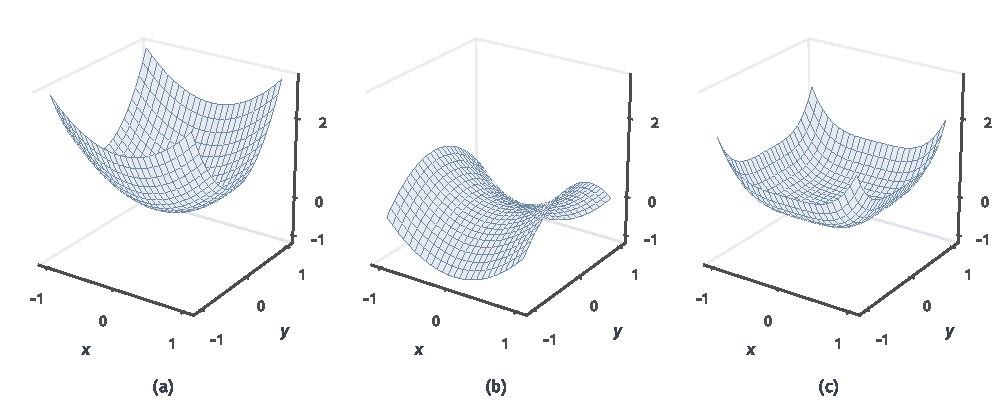
\includegraphics[width=169.0mm]{figures/00-shared/mathematical-preliminaries-upper/00-shared/matplotlib/chapter3-concept-processes/hessian-local-shapes.pdf}
 \caption{同一$[-1,1]^2$范围和纵轴尺度下，三面分别为$x^2+2y^2$、$x^2-y^2$、$x^4+y^4$。原点的Hessian依次为正定、不定、零矩阵；前两者给严格极小与鞍点，第三者虽严格极小却不能由正定判据推出。零Hessian也可能没有极值，例如前述$x^3$，故退化不是一种确定分类。}
 \label{fig:analysis-process-hessian-local-shapes}
\end{figure*}


\FloatBarrier
\section{本章小结}
\label{sec:multivariate-differentiation-chapter-summary}

本章的对象是位置上的量：标量场在每点给出一个数，向量场在每点给出一个与位置同维的向量，一般向量值函数的输出维数可以不同。它们的极限与连续性按输入、输出的范数理解，输出可以逐分量判断，输入的多个坐标却不能拆开逐个检查；沿两条路径得到不同极限能否定极限存在，只查若干条路径则不能证明它存在。

偏导数和方向导数只考察固定的直线。可微要求所有小扰动共用一个线性近似，包括方向随步长改变的扰动；这个近似由偏导数唯一确定。偏导数存在、全部方向导数存在或函数连续，都不单独保证可微；即使全部方向导数组成一个线性映射，仍须满足统一的余项条件。偏导数连续是方便的充分条件，但不是必要条件。

全微分是输入扰动上的线性泛函，梯度是它在所选内积下的表示向量。改变内积会改变梯度的坐标和最陡上升方向，全微分本身不变。沿含于定义域的线段，中值公式把梯度的大小化为有限变化的界；在凸开集上，梯度长度的统一上界恰好就是Lipschitz常数，凸性不能省略。

输出为向量时，微分由Jacobian矩阵表示，它的行是各分量的梯度，列是各输入坐标对输出点的推动。复合映射的Jacobian按计算顺序相乘，标量目标的梯度则由微分的伴随传回输入端。向量增量没有共同的中值点，改用沿线段的积分表示，并由导数的算子范数控制长度。

把微分再用于梯度，得到Hessian与二阶Taylor公式。混合偏导数在连续时可以交换，$C^2$函数的Hessian因而对称。在开集内的驻点处，Hessian正定、负定或不定分别对应严格极小、严格极大和鞍点；半定而退化的情形需要更高阶的信息，边界点和受约束的问题也不在这一判别的范围内。

这些结论都是局部的：可微只保证余项是$o(\lVert\bm h\rVert)$，不说明给定步长下误差有多大。矩阵自变量的微分公式、隐式方程确定的解，以及导数怎样控制误差放大和一阶预测的精度，依次在后面三章展开。

